\documentclass[a4paper, 11pt, oneside]{Thesis}  % Use the "Thesis" style, based on the ECS Thesis style by Steve Gunn
\graphicspath{Figures/}  % Location of the graphics files (set up for graphics to be in PDF format)
\usepackage[square, numbers, comma, sort&compress]{natbib}
\usepackage{verbatim}  % Needed for the "comment" environment to make LaTeX comments
\usepackage{vector}  % Allows "\bvec{}" and "\buvec{}" for "blackboard" style bold vectors in maths
\hypersetup{urlcolor=blue, colorlinks=true}  % Colours hyperlinks in blue, but this can be distracting if there are many links.

\begin{document}
\frontmatter      % Begin Roman style (i, ii, iii, iv...) page numbering

% Set up the Title Page
\title  {The Fundamental Group}
\authors  {\texorpdfstring
            {\href{www.albohessab.weebly.com}{Miliyon T.}}
            {Miliyon T.}
            }
\addresses  {\groupname\\\deptname\\\univname}  % Do not change this here, instead these must be set in the "Thesis.cls" file, please look through it instead
\date       {\today}
\subject    {}
\keywords   {}

\maketitle
%% ----------------------------------------------------------------

\setstretch{1.3}  % It is better to have smaller font and larger line spacing than the other way round

% Define the page headers using the FancyHdr package and set up for one-sided printing
\fancyhead{}  % Clears all page headers and footers
\rhead{\thepage}  % Sets the right side header to show the page number
\lhead{}  % Clears the left side page header

\pagestyle{fancy}  % Finally, use the "fancy" page style to implement the FancyHdr headers

%% ----------------------------------------------------------------
% Declaration Page required for the Thesis, your institution may give you a different text to place here
\clearpage  % Declaration ended, now start a new page

%% ----------------------------------------------------------------
% The "Funny Quote Page"
\pagestyle{empty}  % No headers or footers for the following pages

\null\vfill
% Now comes the "Funny Quote", written in italics
\textit{``Changed and yet the same. I rise again.''}

\begin{flushright}
Jacob Bernoulli
\end{flushright}

\vfill\vfill\vfill\vfill\vfill\vfill\null
\clearpage  % Funny Quote page ended, start a new page
%% ----------------------------------------------------------------

% The Abstract Page
\addtotoc{Abstract}  % Add the "Abstract" page entry to the Contents
\abstract{
\addtocontents{toc}{\vspace{1em}}  % Add a gap in the Contents, for aesthetics

The purpose of this project is to explicitly define the fundamental group and study its properties. The introduction part is just a review section on which we discuss basic set theory, group theory and Topology so that we could have a concrete background.

}

\clearpage  % Abstract ended, start a new page
%% ----------------------------------------------------------------

\setstretch{1.3}  % Reset the line-spacing to 1.3 for body text (if it has changed)

% The Acknowledgements page, for thanking everyone
\acknowledgements{
\addtocontents{toc}{\vspace{1em}}  % Add a gap in the Contents, for aesthetics

First and foremost, I would like to thank the one above, to whom I owe my breath. I can't fully express my gratitude using human made words; therefore, I can only say "Thank you!", and nothing more.

I would not forgive myself if I forget to mention Fikreab Solomon, whom I affectionately call Fiker, for sparking in me an unquenchable thirst for advanced mathematical wisdom, and supporting me with all I requested since my freshman year. I would also like to thank my beloved instructors: Ato Ademe (Gash Ade/Sailor), I would not be exaggerating if I said I have never come across a teacher with your level of spirit and fervor for teaching mathematics. Dr. Yirgalem, you are truly an inspiration, and attending your lectures was nothing short of historical for me. Dr. Yismaw, I would like to
offer heartfelt thanks for supporting and guiding me without tiring. Dr. Zelalem, if it wasn't you who thought me group theory, working on this project would have been equated with climbing \textit{Ras Dashen}. Ato Tesfa, you have molded me into a strong student, as a teacher should do. Dr. Tilahun, your gift of explaining complex concepts in the simplest ways has been invaluable for my success. I would also like to thank my friends, for being there for me, and helping me to be the person that I am today. I am truly thankful for all the fun moments we had, the exuberant knowledge we shared, and the memories we made.

Finally, I would like to thank my advisor, Ato Fikre Bogale, for bringing this beautiful topic in to my insight.

THANK YOU!


\begin{flushright}
Miliyon Tilahun\\
Addis Ababa University\\
Department of Mathematics\\
Email: \texttt{miliyon@ymail.com}
\end{flushright}
}
\clearpage  % End of the Acknowledgements
%% ----------------------------------------------------------------

\pagestyle{fancy}  %The page style headers have been "empty" all this time, now use the "fancy" headers as defined before to bring them back


%% ----------------------------------------------------------------
\lhead{\emph{Contents}}  % Set the left side page header to "Contents"
\tableofcontents  % Write out the Table of Contents

%% ----------------------------------------------------------------
\setstretch{1.5}  % Set the line spacing to 1.5, this makes the following tables easier to read
\clearpage  % Start a new page
\lhead{\emph{Abbreviations}}  % Set the left side page header to "Abbreviations"
\listofsymbols{ll}  % Include a list of Abbreviations (a table of two columns)
{
% \textbf{Acronym} & \textbf{W}hat (it) \textbf{S}tands \textbf{F}or \\
\textbf{LAH} & \textbf{L}ist \textbf{A}bbreviations \textbf{H}ere \\
\textbf{WTS} & \textbf{W}ant \textbf{T}o \textbf{S}how \\
\textbf{QED} & \textbf{Q}uad \textbf{E}tta \textbf{D}emonstrum \\
\textbf{IFF} & \textbf{If} and only I\textbf{f} \\
}

%% ----------------------------------------------------------------
\clearpage  %Start a new page
\lhead{\emph{Symbols}}  % Set the left side page header to "Symbols"
\listofnomenclature{lll}  % Include a list of Symbols (a three column table)
{
% symbol & name \\
$\in$ & Membership in a set \\
$A\times B$ & Cartesian product \\
$\ni$ & Such that \\
$\cap$ & Intersection \\
$\cup$ & Union \\
$\Rightarrow$ & Implies \\
$\Leftrightarrow$ & If an only if \\
$\subset$ & Subset \\
$\emptyset$ & Null set \\
$\exists$ & There exists \\
$\forall$ & For all \\
$\square$ & End of a proof \\
$aH$ & Left coset \\
$Ha$ & Right coset \\
$(G,*)$ & Group \\
$e$ & Identity element \\
$a^{-1}$ & The inverse of a \\
$G/H$ & Quotient group \\
$\lhd$ & Normal subgroup \\
$|G|$ & Number of elements in G\\
$\mathbb{Z}$ & The of Integers \\
$\mathbb{Q}$ & The set of Rational numbers \\
$\mathbb{Q}^\times$ & $\mathbb{Q}-\{0\}$ \\
$\mathbb{R}$ & The set of real numbers \\
$\mathbb{C}$ & The set of complex numbers \\
}
%% ----------------------------------------------------------------
% End of the pre-able, contents and lists of things
% Begin the Dedication page

\setstretch{1.3}  % Return the line spacing back to 1.3

\pagestyle{empty}  % Page style needs to be empty for this page
\dedicatory{For Zer\ldots}

\addtocontents{toc}{\vspace{2em}}  % Add a gap in the Contents, for aesthetics


%% ----------------------------------------------------------------
\mainmatter	  % Begin normal, numeric (1,2,3...) page numbering
\pagestyle{fancy}  % Return the page headers back to the "fancy" style

% Include the chapters of the thesis, as separate files
% Just uncomment the lines as you write the chapters
\lhead{\emph{Introduction}}  % Set the left side page header to "Symbols"
\chapter{Introduction}

In algebraic topology, the fundamental group\footnote{Henri Poincare} is a mathematical group associated to any given pointed topological space that provides a way to determine when two paths, starting and ending at a fixed base point, can be continuously deformed into each other. It records information about the basic shape, or holes, of the topological space. The fundamental group is a topological invariant: homeomorphic topological spaces have isomorphic (the same except name) fundamental group.\\
In order to understand the fundamental group, we need to know some concepts from set theory, group theory and topology. So, we shall review.
\section{Basic Set Theory}
Without set theory it is impossible to study group theory and topology. Of course it is impossible to study mathematics without set theory, as it is the foundation. So let's start to review set theory by giving the intuitive definition of what a set mean.
\begin{definition}
Any well defined collection of object is called a set.
\end{definition}
The objects comprising the set are called its elements or members.
\begin{definition}
A set $A$ is said to be a subset of $B$ or equivalently, $B$ is a superset of $A$, written
$$ A\subset B ~or~ B\supset A$$
iff each elements in $A$ belongs to $B$.
\end{definition}

\begin{definition}[\textbf{Equality}]
Two sets $A$ and $B$ are equal if and only if  $A\subset B$ and $B\subset A$.
\end{definition}
We always use the above definition to prove two sets are equal.
\begin{definition}
A set with no elements in it is called the \textbf{empty set} and  it is denoted by $\emptyset$.
\end{definition}

\begin{remark}
The empty set is a subset of every set.
\end{remark}
\begin{definition}
The \textbf{union} of two sets $A$ and $B$ is defined as
\[
A \cup B = \{x : x \in A \text{ or } x \in B \};
\]
\end{definition}
\begin{definition}
The \textbf{intersection} of $A$ and $B$  is defined by
\[
A \cap B = \{x :  x \in A \text{ and } x \in B \}.
\]
\end{definition}
We can consider a finite union and intersection of more than two sets.  In this case we write
\[
\bigcup_{i = 1}^{n} A_{i} = A_{1} \cup \ldots \cup A_n
\]
and
\[
\bigcap_{i = 1}^{n} A_{i} = A_{1} \cap \ldots \cap A_n
\]
for the union and intersection, respectively, of the sets $A_1, \ldots, A_n$.
\begin{definition}
When two sets have no elements in common, they are said to be \textbf{disjoint}. Two sets $A$ and $B$ are disjoint exactly when $A \cap B = \emptyset$.
\end{definition}
Sometimes we will work within one fixed set $U$, called the \textbf{universal set}.  For any set $A \subset U$, we define the \textbf{complement} of $A$, denoted by $A'$, to be the set
\[
A' = \{ x : x \in U \text{ and } x \notin A \}.
\]
The \textbf{difference} of two sets $A$ and $B$ is defined by
\[
A \setminus B = A \cap B'  = \{ x : x \in A \text{ and } x \notin B \}.
\]

\begin{proposition}
Let $A$, $B$, and $C$ be sets. Then
\begin{enumerate}

\rm\item\it
$A \cup A = A$, $A \cap A = A$, and $A \setminus A = \emptyset$;

\rm\item\it
$A \cup \emptyset = A$ and $A \cap \emptyset = \emptyset$;

\rm\item\it
$A \cup (B \cup C) = (A \cup B) \cup C$ and  $A \cap (B \cap C) = (A \cap B) \cap C$;

\rm\item\it
$A \cup B = B \cup A$ and $A \cap B = B \cap A$;

\rm\item\it
$A \cup (B \cap C) = (A \cup B) \cap (A \cup C)$;

\rm\item\it
$A \cap (B \cup C) = (A \cap B) \cup (A \cap C)$.

\end{enumerate}
\end{proposition}
The following theorem is a very important theorem in set theory due to British mathematician Augustus De Morgan.
\begin{theorem}[\textbf{De Morgan's Laws}]
Let $A$ and $B$ be sets. Then
\begin{enumerate}

\rm\item\it
$(A \cup B)' = A' \cap B'$;

\rm\item\it
$(A \cap B)' = A' \cup B'$.

\end{enumerate}
\end{theorem}
\begin{proof}
(1)
We must show that $(A \cup B)' \subset A' \cap B'$ and $(A \cup B)' \supset A' \cap B'$. Let $x \in (A \cup B)'$.  Then $x \notin A \cup B$. So $x$ is neither in $A$ nor in $B$, by the definition of the union of sets.  By the definition of the complement, $x \in A'$ and $x \in B'$.  Therefore, $x \in A' \cap B'$ and we have $(A \cup B)' \subset A' \cap B'$.

To show the reverse inclusion, suppose that $x \in A' \cap B'$.  Then $x \in A'$ and $x \in B'$, and so $x \notin A$ and $x \notin B$.  Thus $x \notin A \cup B$ and so $x \in (A \cup B)'$.  Hence, $(A \cup B)' \supset A' \cap B'$ and so $(A \cup B)' = A' \cap B'$.

The proof of (2) is similar.
\end{proof}

\begin{definition}
Given sets $A$ and $B$, we can define a new set $A \times B$, called the \textbf{Cartesian product}\footnote{Rene Descartes} of $A$ and $B$, as a set of ordered pairs.  That is,
$$
A \times B = \{ (a,b) : a \in A \text{ and } b \in B \}.
$$
\end{definition}

If $A = A_1 = A_2 = \cdots = A_n$, we often write $A^n$ for $A \times \cdots \times A$ (where $A$ would be written $n$ times).   For example, the set ${\mathbb R}^3$ consists of all of 3-tuples of real numbers.
\begin{definition}
Subsets of $A \times B$ are called \textbf{relations}.
\end{definition}
\begin{definition}
A \textbf{mapping} or \textbf{function} $f \subset A \times B$ from a set $A$ to a set $B$ to be the special type of  relation in which for each element $a \in A$ there is a unique element $b \in B$ such that $(a, b) \in f$; that means for every element in $A$, $f$ assigns a unique element in $B$.  We usually write $f:A \rightarrow B$ or $A \stackrel{f}{\rightarrow} B$.  Instead of writing down ordered pairs  $(a,b) \in A \times B$, we write $f(a) = b$ or $f : a \mapsto b$.  The set  $A$ is called the \textbf{domain} of $f$ and
\[
f(A) = \{ f(a) : a \in A \} \subset B
\]
is called the \textbf{range} or \textbf{image} of $f$.
\end{definition}
We can think of the elements in the function's domain as input values and the elements in the function's range as output values.

A relation cannot be a mapping because it is not well-defined. A relation is \textbf{well-defined} if each element in the domain is assigned to a \textbf{unique} element in the range.

If $f:A \rightarrow B$ is a map and the image of $f$ is $B$, i.e., $f(A) = B$, then $f$ is said to be \textbf{onto} or \textbf{surjective}. In other words, if there exists an $a \in A$ for each $b \in B$ such that $f(a) = b$, then $f$ is onto. A map is \textbf{one-to-one} or \textbf{injective} if $a_1 \neq a_2$ implies $f(a_1) \neq f(a_2)$.  Equivalently, a function is one-to-one if $f(a_1) = f(a_2)$ implies $a_1 = a_2$.  A map that is both one-to-one and onto is called \textbf{bijective}.

\begin{proposition}
Let $f : A \rightarrow B$, $g : B \rightarrow C$, and $h : C \rightarrow D$. Then
\begin{enumerate}

\rm\item\it
The composition of mappings is associative; that is, $(h \circ g) \circ f = h \circ (g \circ f)$;

\rm\item\it
If $f$ and $g$ are both one-to-one, then the mapping $g \circ f$ is one-to-one;

\rm\item\it
If $f$ and $g$ are both onto, then the mapping $g \circ f$ is onto;

\rm\item\it
If $f$ and $g$ are bijective, then so is $g \circ f$.

\end{enumerate}
\end{proposition}

If $S$ is any set, we will use $id_S$ or $id$ to denote the \textbf{identity mapping} from $S$ to itself.  Define this map by $id(s) = s$ for all $s \in S$.  A map $g: B \rightarrow A$ is an \textbf{inverse mapping} of $f: A \rightarrow B$ if $g \circ f = id_A$ and $f \circ g = id_B$; in other words, the inverse function of a function simply "undoes" the function.   A map is said to be \textbf{invertible} if it has an inverse.  We usually write $f^{-1}$ for the inverse of $f$.


\begin{theorem}
A mapping is invertible if and only if it is both one-to-one and onto.
\end{theorem}

\begin{proof}
Suppose first that $f:A \rightarrow B$ is invertible with inverse $g: B \rightarrow A$. Then $g \circ f = id_A$ is the identity map; that is, $g(f(a)) = a$. If $a_1, a_2 \in A$ with $f(a_1) = f(a_2)$, then $a_1 = g(f(a_1)) = g(f(a_2)) = a_2$.  Consequently, $f$ is one-to-one.  Now suppose that $b \in B$. To show that $f$ is onto, it is necessary to find an $a \in A$ such that $f(a) = b$, but $f(g(b)) = b$ with $g(b) \in A$. Let $a = g(b)$.

Now assume the converse; that is, let $f$ be bijective.  Let $b \in B$.  Since $f$ is onto, there exists an $a \in A$ such that $f(a) = b$.  Because $f$ is one-to-one, $a$ must be unique. Define $g$ by letting $g(b) = a$.  We have now constructed the inverse of $f$.
\end{proof}

The review that we have seen so far is just to define an equivalence relation. It is the most important concept in this section that we need for our understanding of the fundamental group.

\begin{definition}
An \textbf{equivalence relation} on a set $X$ is a relation $R \subset X \times X$ such that
\begin{description}
  \item[Reflexive:] $(x, x) \in R$ for all $x \in X$.
  \item[Symmetric:] $(x, y) \in R$ implies $(y, x) \in R$.
  \item[Transitive:] $(x, y)$ and $(y, z) \in R$ imply $(x, z) \in R$.
\end{description}
\end{definition}

A \textbf{partition} ${\mathcal P}$ of a set $X$ is a collection of nonempty sets $X_1, X_2, \ldots$ such that $X_i \cap X_j = \emptyset$ for $i  \neq j$ and $\bigcup_k X_k = X$. Let $\sim$ be an equivalence relation on a set $X$ and let $x \in X$.  Then $[x] = \{ y \in X : y \sim x \}$ is called the \textbf{equivalence class} of $x$.

The important thing about an equivalence relation is that it gives rise to a partition via equivalence classes.  Also, whenever a partition of a set exists, there is some natural  underlying equivalence relation, as the following theorem demonstrates.

\medskip

\begin{theorem}
Given an equivalence relation $\sim$ on a set $X$, the equivalence classes of $X$ form a partition of $X$.  Conversely, if ${\mathcal P} = \{ X_i\}$ is a partition of a set $X$, then there is an equivalence relation on $X$ with equivalence classes $X_i$.
\end{theorem}

\begin{proof}
Suppose there exists an equivalence relation $\sim$ on the set $X$.  For any $x \in X$, the reflexive property shows that $x \in [x]$ and so $[x]$ is nonempty.  Clearly $X = \bigcup_{x \in X} [x]$.  Now let $x, y \in X$. We need to show that either $[x] = [y]$ or $[x] \cap [y] = \emptyset$.  Suppose that the intersection of $[x]$ and $[y]$ is not empty and that $z \in [x] \cap [y]$. Then $z \sim x$ and $z \sim y$.  By symmetry and transitivity $x \sim y$; hence, $[x] \subset [y]$.  Similarly, $[y] \subset [x]$ and so $[x] = [y]$.  Therefore, any two equivalence classes are either disjoint or exactly the same.

Conversely, suppose that ${\mathcal P} = \{X_i\}$ is a partition of a set $X$.  Let two elements be equivalent if they are in the same partition. Since $x\sim x$, the relation is reflexive.  If $x$ is in the same partition as $y$, then $y$ is in the same partition as $x$, so $x \sim y$ implies $y \sim x$.  Finally, if $x$ is in the same partition as $y$ and $y$ is in the same partition as $z$, then $x$ must be in the same partition as $z$, and transitivity holds.
\end{proof}
\newpage
\section{Basic Group Theory}
As we have mentioned in the abstract our aim is to understand the fundamental group. So, what is the fundamental group? Well, it is a mathematical group. What is a mathematical group? To answer this question and to see some basic results which are very helpful for our understanding of the fundamental group  we are forced to review group theory. We begin our revision by defining a Group in mathematics.

\begin{definition}[\textbf{Group}]
An algebraic structure with one binary operation $(G,\Delta)$ is called a group iff\footnote{For definition if and iff are the same} the following four conditions are satisfied
\begin{enumerate}
  \item $\forall a,b\in G \Rightarrow a\Delta b \in G \qquad \qquad \text{Closure}$
  \item $\forall a,b,c \in G \Rightarrow a\Delta (b\Delta c)=(a\Delta b)\Delta c\qquad \text{Associative}$
  \item $\exists e\in G \ni  a\Delta e=e\Delta a \qquad \forall a \in G\qquad \text{Identity}$
  \item $\forall a\in G ,\exists a^{-1}\in G \ni a\Delta a^{-1} =e=a^{-1}\Delta a \qquad \text{Inverse}$
\end{enumerate}
\end{definition}Moreover if $\Delta$ is commutative the group $G$ is called an \textbf{abelian group}.\\
The above four conditions are called group axioms. In our definition of a mathematical group there is a word "algebraic structure". Algebraic structure is nothing but a non empty set together with one or more finitary operations defined on it. Hence we can rewrite our definition of a mathematical group as \textit{a non empty set with one binary operation defined on it.} From now on we designate $a\Delta b$ by $ab$.
\begin{example}
Here are some examples of groups.
\begin{itemize}
  \item  $(\mathbb{Z},+)$ The set of integers with addition is a group.
  \item $(\mathbb{Q},+)$ The set of rational numbers with addition is a group.
  \item $(\mathbb{C}^\times,\times)$ The set of non zero complex numbers with the usual multiplication is a group.
\end{itemize}
\end{example}
\begin{conj}
There exists a group structure in the set of prime numbers.
\end{conj}

\begin{lemma}\label{uniquee}
The identity element in a group is unique.
\end{lemma}
\begin{proof}
Suppose that $e$ and $e'$ are both identities in $G$. Then $eg = ge =g$ and $e'g = ge' = g$ for all $g \in G$. We need to show that $e =e'$. If we think of $e$ as the identity, then $ee' = e'$; but if $e'$ is the identity, then $ee' = e$. Combining these two equations, we have $e = ee' = e'$.
\end{proof}

\begin{lem}[\textbf{Cancellation Law}]\label{cancelem}
If $G$ is a group and $a, b, c \in G$, then $ba = ca$ implies $b = c$
and $ab = ac$ implies $b = c$.
\end{lem}
\begin{proof}
Multiplying the equations by the appropriate inverse gives us the desired result.
\end{proof}

\begin{lemma}\label{uniquei}
If $g$ is any element in a group $G$, then the inverse of $g$, $g^{-1}$, is unique.
\end{lemma}
\begin{proof}
Suppose $g'$ and $g''$ are inverses of $g\in G$. WTS $g'=g''$. Now, since $g'$ is the inverse of $g$ we have $gg'=e$ and we have $gg''=e$ as $g''$ is the inverse of $g$. From the uniqueness of the identity element in a group we conclude that $gg'=gg''$. Hence $g'=g''$ by lemma (\ref{cancelem}).
\end{proof}
\begin{remark}
We denote the unique inverse of $g$ by $g'$.
\end{remark}

\begin{proposition}[\textbf{Socks Shoe}]
Let $G$ be a group. If $a, b \in G$, then $(ab)^{-1} = b^{-1}a^{-1}$.
\end{proposition}


\begin{proof}
Let $a, b \in G$. Then $abb^{-1}a^{-1} = aea^{-1} = aa^{-1} = e$. Similarly, $b^{-1}a^{-1}ab = e$. But by lemma (\ref{uniquei}), inverses are unique; hence, $(ab)^{-1} = b^{- 1}a^{-1}$.
\end{proof}


\begin{proposition}
Let $G$ be a group.  For any $a \in G$, $(a^{-1})^{-1} = a$.
\end{proposition}


\begin{proof}
Observe that $a^{-1} (a^{-1})^{-1} = e$. Consequently, multiplying
both sides of this equation by $a$, we have
$$ (a^{-1})^{-1} = e (a^{-1})^{-1} = a a^{-1} (a^{-1})^{-1} = ae = a.$$
\end{proof}
It makes sense to write equations with group elements and group operations. If $a$ and $b$ are two elements in a group $G$, does there exist an element $x \in G$ such that $ax = b$? If such an $x$ does exist, is it unique? The following proposition answers both of these questions.


\begin{proposition}\label{group_equations}
Let $G$ be a group and $a$ and $b$ be any two elements in $G$. Then the equations $ax = b$ and $xa = b$ have unique solutions in $G$.
\end{proposition}


\begin{proof}
Suppose that $ax = b$. We must show that such an $x$ exists. Multiplying both sides of $ax = b$ by $a^{-1}$, we have $x = ex = a^{-1}ax = a^{-1}b$.


To show uniqueness, suppose that $x_1$ and $x_2$ are both solutions of $ax = b$; then $ax_1 = b = ax_2$. So $x_1 = a^{-1}ax_1 = a^{-1}ax_2 = x_2$. The proof for the existence and uniqueness of the solution of $xa = b$ is similar.
\end{proof}

\begin{definition}[\textbf{Subgroup}]
Let G be a group and $\emptyset \neq H\subset G$ we say that $H$ is a subgroup of $G$ if $H$ by itself is a group.
We denote $H$ a subgroup of $G$ by $H\lesssim G$.
\end{definition}

\begin{example}
Let $H=\{ \pm1,\pm i\}$, then $H$ with the usual multiplication $(H,\times)$ is a subgroup of $(\mathbb{C^{\times}},\times)$.
\end{example}
\begin{proposition}[\textbf{Subgroup test}]\label{subtest}
Let G be a group and $\emptyset \neq H\subset G$ we say that $H$ is a subgroup of $G$ iff
\begin{enumerate}
  \item $\forall a,b\in H \Rightarrow a\Delta b \in H \qquad \qquad \text{Closure}$
  \item $\forall a \in H,\exists a^{-1}\in H \ni a\Delta a^{-1} =e=a^{-1}\Delta a \qquad \text{Inverse}$
\end{enumerate}
\end{proposition}

\begin{definition}[\textbf{Normal Subgroup}]
A subgroup $N$ of a group $G$ is \textbf{normal} in G if $gN =Ng$ for all $g \in G$. We denote $N$ is a normal subgroup of $G$ by $N\lhd G$.
\end{definition}

\begin{remark}
$H$ is normal in $G$ doesn't mean $ah=ha$ for $a\in G$ and $h\in H$. This is not what normality mean; rather, it means if $a\in G$ and $h\in H$, then there exists elements $h'$ and $h''$ in $H$ such that $ah=h'a$ and $ha=ah''$.
\end{remark}
\begin{proposition}
A subgroup $H$ of $G$ is normal in $G$ iff $xHx^{-1}\subset H$ for all $x\in G$.
\end{proposition}
\begin{proof}
If $H$ is normal in $G$, then for any $x\in G$ and $h\in H$ there is $h'\in H$ such that $xh=h'x.$ Thus, $h'=xhx^{-1}$ and therefore $xHx^{-1}\subset H$.\\
Conversely, if $xHx^{-1}\subset H$ for all $x\in G$, then letting $x=a$, we have $aHa^{-1}\subset H$ or $aH\subset Ha$. On the other hand, letting $x=a^{-1}$ we have $a^{-1}H(a^{-1})^{-1}=a^{-1}Ha\subset H$ or $Ha\subset aH.$
\end{proof}
\begin{definition}[\textbf{Cosets}]
Let $G$ be a group and $H$ a subgroup of $G$.  We define a \textbf{left  coset} of $H$ with \textbf{representative} $g \in G$ to be the set $gH = \{ gh : h \in H \}.$ \textbf{Right cosets} can be defined similarly by $Hg = \{ hg : h \in H \}.$
\end{definition}
If left and right cosets coincide or if it is clear from the context to which type of coset that we are referring, we will use the word \textbf{coset} without specifying left or right.
\begin{lemma}\label{coslemma}
 $aH = bH$ if and only if $a \in bH$.
\end{lemma}
\begin{proof}
 If $aH=bH$, then $a = ae \in aH=bH$. Conversely, if $a \in bH$ we have $a = bh$ where $h \in H$, and therefore $aH = (bh)H = b(hH) = bH$.
\end{proof}

The coset of a group partitions the group as the following proposition demonstrates.
\newpage
\begin{proposition}
Let $H$ be a subgroup of a group $G$.  Then the left cosets of $H$ in $G$ partition $G$.  That is, the group $G$ is the disjoint union of the left cosets of $H$ in $G$.
\end{proposition}

\begin{proof}
Let $g_1 H$ and $g_2 H$ be two cosets of $H$ in $G$.  We must show that either $g_1 H \cap g_2 H = \emptyset$ or $g_1 H = g_2 H$.  Suppose that $g_1 H \cap g_2 H \neq \emptyset$ and $a \in g_1 H \cap g_2 H$.  Then by the definition of a left coset, $a = g_1 h_1 = g_2 h_2$ for some elements $h_1$ and $h_2$ in $H$.  Hence, $g_1 = g_2 h_2 h_1^{-1}$ or $g_1 \in g_2 H$.  By lemma~\ref{coslemma}, $g_1 H = g_2 H$.
\end{proof}

The following theorem is the most important result in group theory. I rather forget about the project than to proceed without mentioning it.

\begin{theorem}[Lagrange]
Let $G$ be a finite group and let $H$ be a subgroup of $G$.  Then $|G|/|H| = [G : H]$ is the number of distinct left cosets of $H$ in $G$.  In particular, the number of elements in $H$ must divide the number of elements in $G$.
\end{theorem}

\begin{proof}
The group $G$ is partitioned into $[G : H]$ distinct left cosets.  Each left coset has $|H|$ elements; therefore, $|G| = [G : H] |H|$.
\end{proof}

\begin{proposition}
Let $N\lhd G$. The set $G/N = \{ aN:a\in G\}$ is a group under the operation $(aN)(bN)=(ab)N$.
\end{proposition}
\begin{proof}
First of all we have to show the operation $(aN)(bN)=(ab)N$ is well defined. i.e. We need to show the "multiplication" is independent of the choice of representative. For $a,b,c,d\in G$ let $aN=bN$ and $cN=dN$. Then by Lemma (\ref{coslemma}) $a=bn_1$ and $c=dn_2$ for some $n_1,n_2\in N$. Hence $$ acN=bn_1dn_2N=bn_1dN=bn_1Nd=bNd=bdN$$.
To show the associativity $(aNbN)cN=(ab)NcN=(abc)N=aN(bcN)=aN(bNcN).$ The identity element is $eN=N$. For any $a\in G$ $a^{-1}N$ is the inverse of $aN$.
\end{proof}
We have already used the fact that $N$ is normal while showing the well defined-ness of the "multiplication". But let's see what would happen if $N$ was not normal. Thus $aN\neq Na \Rightarrow N\neq aNa^{-1} \Rightarrow \exists n\in N \ni ana^{-1}\notin N $. Now, take cosets $aN$ and $a^{-1}N$ by our definition of the "multiplication" $(aN)(a^{-1}N)=eN$ but we can show this not true. Take for example $n,e\in N$ thus $ana^{-1}\notin N$.
\begin{definition}
The group $G/N$ in the preceding proposition is called quotient group.
\end{definition}

\begin{definition}[\textbf{Homomorphism}]
A homomorphism between groups\footnote{\'{E}variste Galois} $(G, \cdot)$ and $(H, \circ)$ is a map $\phi : G \rightarrow H$ such that
\[
\phi( g_1 \cdot g_2 ) = \phi( g_1 ) \circ \phi( g_2 )
\]
\end{definition}

\begin{example}
Let $G$ be a group and $g \in G$. Define a map $\phi : {\mathbb Z}
\rightarrow G$ by $\phi( n ) = g^n$. Then $\phi$ is a group
homomorphism, since
\[
\phi( m + n ) = g^{ m + n} = g^m g^n = \phi( m ) \phi( n ).
\]
This homomorphism maps ${\mathbb Z}$ onto the cyclic subgroup of $G$
generated by $g$.
\end{example}

If $\phi$ is injective, $\phi$ is a monomorphism. If $\phi$ is surjective, $\phi$ is an epimorphism. If $\phi$ is bijective, $\phi$ is a isomorphism.

\begin{example}
Consider the group $(\mathbb{R},+)$ and $(\mathbb{R}^+,\cdot)$. Define $f:\mathbb{R}\rightarrow \mathbb{R}^+$ by $f(x)=e^x$. To show $f$ is a homomorphism\\ Let $a,b\in \mathbb{R},\qquad f(ab)=f(a+b)=e^{a+b}=e^a\cdot e^b=f(a)\cdot f(b),$\\
One to oneness,$\qquad f(x)=f(y) \Rightarrow e^x=e^y$
$$ \Rightarrow x=y.$$
Ontoness,$\qquad$ let $b\in \mathbb{R}^+$, Take $a=\ln b \in \mathbb{R}$. Then
$f(a)=e^{\ln b}=b.$
Hence $f$ is an isomorphism.
\end{example}
\begin{proposition}
Let $\phi : G_1 \rightarrow G_2$ be a homomorphism of groups. Then
\begin{enumerate}

\rm \item \it
If $e$ is the identity of $G_1$, then $\phi( e)$ is the identity of
$G_2$;

\rm \item \it
For any element $g \in G_1$, $\phi( g^{-1}) = [\phi( g )]^{- 1}$;
\end{enumerate}
\end{proposition}

\begin{proof}
(1)
Suppose that $e$ and $e'$ are the identities of $G_1$ and $G_2$,
respectively; then
\[
e' \phi(e) = \phi(e) = \phi(e e) = \phi(e) \phi(e).
\]
By right cancellation, $\phi(e) = e'$.

(2)
This statement follows from the fact that
$$
\phi( g^{-1}) \phi(g) = \phi(g^{-1} g) = \phi(e) = e'.
$$
\end{proof}

\begin{definition}
Let $f : G \rightarrow H$ be a homomorphism of groups, \textbf{kernel} of $f$ is given by
$$ kerf=\{a\in G:f(a)=e_H\}$$
\end{definition}

\begin{lemma}
$kerf$ is a subgroup of $G$.
\end{lemma}

\begin{proof}
Let $x,y\in kerf$. Then $f(x)=e_H$ and $f(y)=e_H$. Now $$f(xy)=f(x)f(y)=e_He_H=e_H.$$ And $f(x^{-1})=(f(x))^{-1}=e_H.$ Hence $xy$ and $x^{-1}$ are in $kerf$. By lemma (\ref{subtest}) we can conclude that $kerf$ is a subgroup of $G$.
\end{proof}

In fact, kernel of a homomorphism is a normal subgroup.
\begin{proposition}
Let $f : G \rightarrow H$ be a homomorphism of groups, $kerf\lhd G$.
\end{proposition}

\begin{proof}
It suffices to show that $\forall g\in G$, $gkerf g^{-1}\subset kerf.$
\end{proof}

\begin{theorem}
Let $f : G \rightarrow H$ be a homomorphism of groups, $f$ is a monomorphism iff $kerf=\{e_G\}$.
\end{theorem}
\begin{proof}
Suppose $f$ is a monomorphism. WTS $kerf=\{e_G\}$. let $a\in kerf$, then $f(a)=e_H$. We know that $f(e_G)=e_H$. Since $f$ is injective $a=e_G$. Conversely, suppose $kerf=\{e_G\}$.
\begin{align*}
 Let~f(a)=f(b) &\Rightarrow f(a)f^{-1}(b)=f(b)f^{-1}(b)=e_H\\
               &\Rightarrow f(a)f(b^{-1})=e_H\\
               &\Rightarrow f(ab^{-1})=e_H
\end{align*}
This implies $ab^{-1}\in kerf={e_G}$. Thus $ab^{-1}=e_G\Rightarrow a=b.$ Hence $f$ is injective.
\end{proof}
\newpage
\section{Basic Topology}
Topology is the mathematical study of the properties that are preserved through deformations, twistings, and stretchings of objects. Informally, we can also define topology as a geometry of sets.


\begin{definition}
A \textit{\textbf{topology}} on a set $X$ is a collection $\tau$ of subsets of a non empty set $X$ satisfying the following axioms:
\begin{enumerate}
  \item $\emptyset$ and $X$ are in $\tau$.
  \item The union of any number of sets in $\tau$ is in $\tau$.
  \item The intersection of any two sets in $\tau$ is in $\tau$.
\end{enumerate}
The members of $\tau$ are then called $\tau - open~sets,$ or simply open sets.
\end{definition}

\begin{definition}
A \textbf{neighborhood} of a point $x$ in a topological space is a subset $N$, such that there is an open subset $U$ satisfying $x\in U\subset N$.
\end{definition}
An open neighborhood of $x$ is simply an open subset containing $x$. If $N$ is a neighborhood of $x$, then any subset bigger than $N$ is also a neighborhood of $x$. Moreover, a finite intersection of neighborhoods of $x$ is still a neighborhood of $x$. More generally, a subset $N$ is a neighborhood of a subset $A$, if there is an
open subset $U$ satisfying $A\subset U\subset N$.

\begin{definition}
An ordered pair $(X,\tau)$ consisting of a set $X$ and a topology $\tau$ is called a \textbf{topological space}.
\end{definition}


\begin{example}\label{example1}
Let $O$ denotes the class of all open sets of real numbers. Then $O$ is a topology on $\mathbb{R}$ (The \textbf{usual topology} on $\mathbb{R}$).
\end{example}



\begin{example}\label{example2}
Let $D$ denotes the class of all subsets of $X$. Clearly, $D$ satisfies the above axioms.
This topology is called the \textbf{discrete topology}. i.e. the pair $(X,D)$ is called a discrete topological space or simply a discrete space.
\end{example}

\begin{example}\label{example3}
The class $\jmath =\{X,\emptyset\}$ consisting of $X$ and $\emptyset$ alone is itself a topology on $X$. It is called the \textbf{indiscrete topology}. i.e. the pair $(X,\jmath)$ is called a indiscrete topological space or simply a indiscrete space.
\end{example}

\begin{example}\label{example4}
Let $\tau $ denote the class of all subsets of $X$ whose complements are finite together with the empty set $\emptyset$. This class $\tau $ is also a topology on $X$. This class $\tau$ is called cofinite topology or the $T_1-$topology on $X$.
\end{example}

\begin{proposition}
For any two topologies $\tau_1$ and $\tau_2$ on $X$ their intersection $\tau_1\cap \tau_2$ is also a topology on $X$.
\end{proposition}

\begin{proof}
Suppose $\tau_1$ and $\tau_2$ are topologies on $X$. By axiom $1$ $X$ and $\emptyset$ belongs to both $\tau_1$ and $\tau_2$; hence $X$ and $\emptyset$ each belongs to the intersection $\tau_1\cap\tau_2$. Furthermore if $G_1,G_2\in \tau_1\cap\tau_2$, then in particular $G_1,G_2\in \tau_1$ and $G_1,G_2\in \tau_2$. But since $\tau_1$ and $\tau_2$ are topologies $G_1\cap G_2\in \tau_1$ and $G_1\cap G_2\in \tau_2$. Accordingly, $G_1\cap G_2\in \tau_1\cap\tau_2$
\end{proof}

But the union of two topologies $\tau_1$ and $\tau_2$ on $X$ is not necessarily a topology on $X$.
To illustrate this let's look at the following example.
\begin{example}
Consider $\tau_1=\{X,\emptyset,\{a\}\}$ and $\tau_2=\{X,\emptyset,\{b\}\}$ is a topology on $X=\{a,b,c\}$. But the union $$ \tau_1\cup\tau_2=\{X,\emptyset,\{a\},\{b\}\} $$
$\tau_1 \cup \tau_2$ is not a topology on $X$. Because it fails to satisfy axiom 2 which says that the union of members of a topology is also a member of a that topology.
\end{example}

Let $A$ be a non-empty subset of a topological space $(X,\tau)$. The class $\tau_A$ of all intersections of $A$ with $\tau-$open subsets of $X$ is a topology on $A;$
$$\tau_A=\{A\cap G:G\in \tau\}$$
it is called a relative topology on $A$ or a relativization of $\tau$ to $A$.
\begin{proposition}
$\tau_A=\{A\cap G:G\in \tau\}$ is a topology on $A$.
\end{proposition}

\begin{proof}
Since $\tau$ is a topology, $X$ and $\emptyset$  belong to $\tau$. Hence $A\cap X=A$ and $A \cap \emptyset=\emptyset$ both belong to $\tau_A$ hence axiom $1$.

Now let $\{H_i: i\in I\}$ be subclass of $\tau_A$. By definition for each $i\in I$ $ \exists $ a $\tau$-open set $G_i$ such that $H_i=A\cap G_i$. By the distributive law of intersection over union,
$$\cup_iH_i=\cup_i(A\cap G_i)=A\cap(\cup_iG_i)$$
But $\bigcup_iG_i\in \tau$ as it is the union of $\tau$-open sets; hence $\bigcup_iH_i\in \tau_A$. Thus $\tau_A$ satisfies axiom $2$.

Now suppose $H_1,H_2 \in \tau_A$. Then $\exists G_1,G_2\in \tau$ such that $H_1=A\cap G_1$ and $H_2=A\cap G_2$. But $G_1\cap G_2\in \tau$ since $\tau$ is a topology. Hence
$$H_1\cap H_2=(A\cap G_1)\cap(A\cap G_2)=A\cap(G_1\cap G_2)$$
belongs to $\tau_A$. Hence $\tau_A$ satisfies axiom $3$ and is a topology on $A$.
\end{proof}

\begin{definition}[\textbf{Subspace}]
The topological space $(A,\tau_A)$ is called a subspace of $(X,\tau)$.
\end{definition}

\begin{example}
Consider the topology
$$\tau=\{X,\emptyset,\{a\},\{c,d\},\{a,c,d\},\{b,c,d,e\}\}$$
on $X=\{a,b,c,d,e\}$ and the subset $A=\{a,d,e\}$ of $X$ is a topology on $X=\{a,b,c\}$. Observe that
\begin{align*}
X\cap A=A, \qquad \{a\}\cap A=\{a\}, \qquad \{a,c,d\}\cap A=\{a,d\} \\
\emptyset\cap A=\emptyset, \qquad \{c,d\}\cap A=\{d\}, \qquad \{b,c,d,e\}\cap A=\{d,e\}
\end{align*}
\end{example}

\begin{definition}[\textbf{Basis}]
Let $(X,\tau)$ be a topological space. A topological basis on a set $X$ is a collection $\mathcal{B}$ of subsets of $X$, such that
\begin{enumerate}
  \item If $x\in X$, then $x\in B$ for some $B\in \mathcal{B}$.
  \item If $x\in B_1\cap B_2$ and $B_1\cap B_2\in \mathcal{B}$, then $x\in B\subset B_1\cap B_2$ for some $B\in \mathcal{B}.$
\end{enumerate}
\end{definition}

\begin{example}
On any set $X$, the collections of all subsets, all finite subsets, and all single point subsets are topological bases. The collection $\{\emptyset, X\}$ is also a topological basis.
\end{example}

\begin{lemma}\label{lemmabasis}
Suppose a collection $\mathcal{B}$ satisfies the first condition and
$$B_1, B_2 \in \mathcal{B} \qquad \Rightarrow \qquad B_1\cap B_2\in \mathcal{B} ~or~ B_1\cap B_2=\emptyset.$$
\end{lemma}

\begin{example}
The collection $\mathcal{B}=\{\{1\}, \{4\}, \{1, 2\}, \{1, 3\}\}$ of subsets of $X = \{1, 2, 3, 4\}$ is
a topological basis by lemma (\ref{lemmabasis}). However, the collection $S = \{\{4\}, \{1, 2\}, \{1, 3\}\}$ is not
a topological basis. It violates condition $2$ with $x = 1, B_1 = \{1, 2\}, B_2 = \{1, 3\}$.
\end{example}

\medskip

\begin{definition}
If $A$ is a subset of the topological space X. A point $p\in X$ is a limit point (or "cluster point," or "point of accumulation") of A iff every open set $G$ containing $p$ contains a point of $A$ diffent from $p$ that is
$$ G~open~,p\in G \qquad \Rightarrow \qquad (G\setminus\{p\})\cap A\neq \emptyset $$
\end{definition}


\begin{definition}
A subset $A$ of a topological space $X$ is said to be closed if the set $A'$ is open.
\end{definition}

\begin{example}
$X$ and $\emptyset$ are closed because their complements ($\emptyset$ and $X$) are open.
\end{example}

\begin{definition}
Let $X$ and $Y$ be topological spaces. A function $f : X \rightarrow Y$ is said to be continuous if for each open subset $V$ of $Y$, the set $f^{-1}(V)$ is an open subset of $X$.
\end{definition}

\begin{example}
Consider the following topologies on $X=\{ a,b,c\}$ and $Y=\{x,y,z\}$ respectively: $\tau =\{X,\emptyset,\{a\},\{a,c\},\{a,b,c\}\}$, $\tau^*=\{Y,\emptyset,\{x\},\{y\},\{x,y\},\{y,z\}\}$ Also consider the functions $f:X\rightarrow Y$ and $g:X\rightarrow Y$ defined by the diagrams
\begin{figure}[hbt!]
\centering
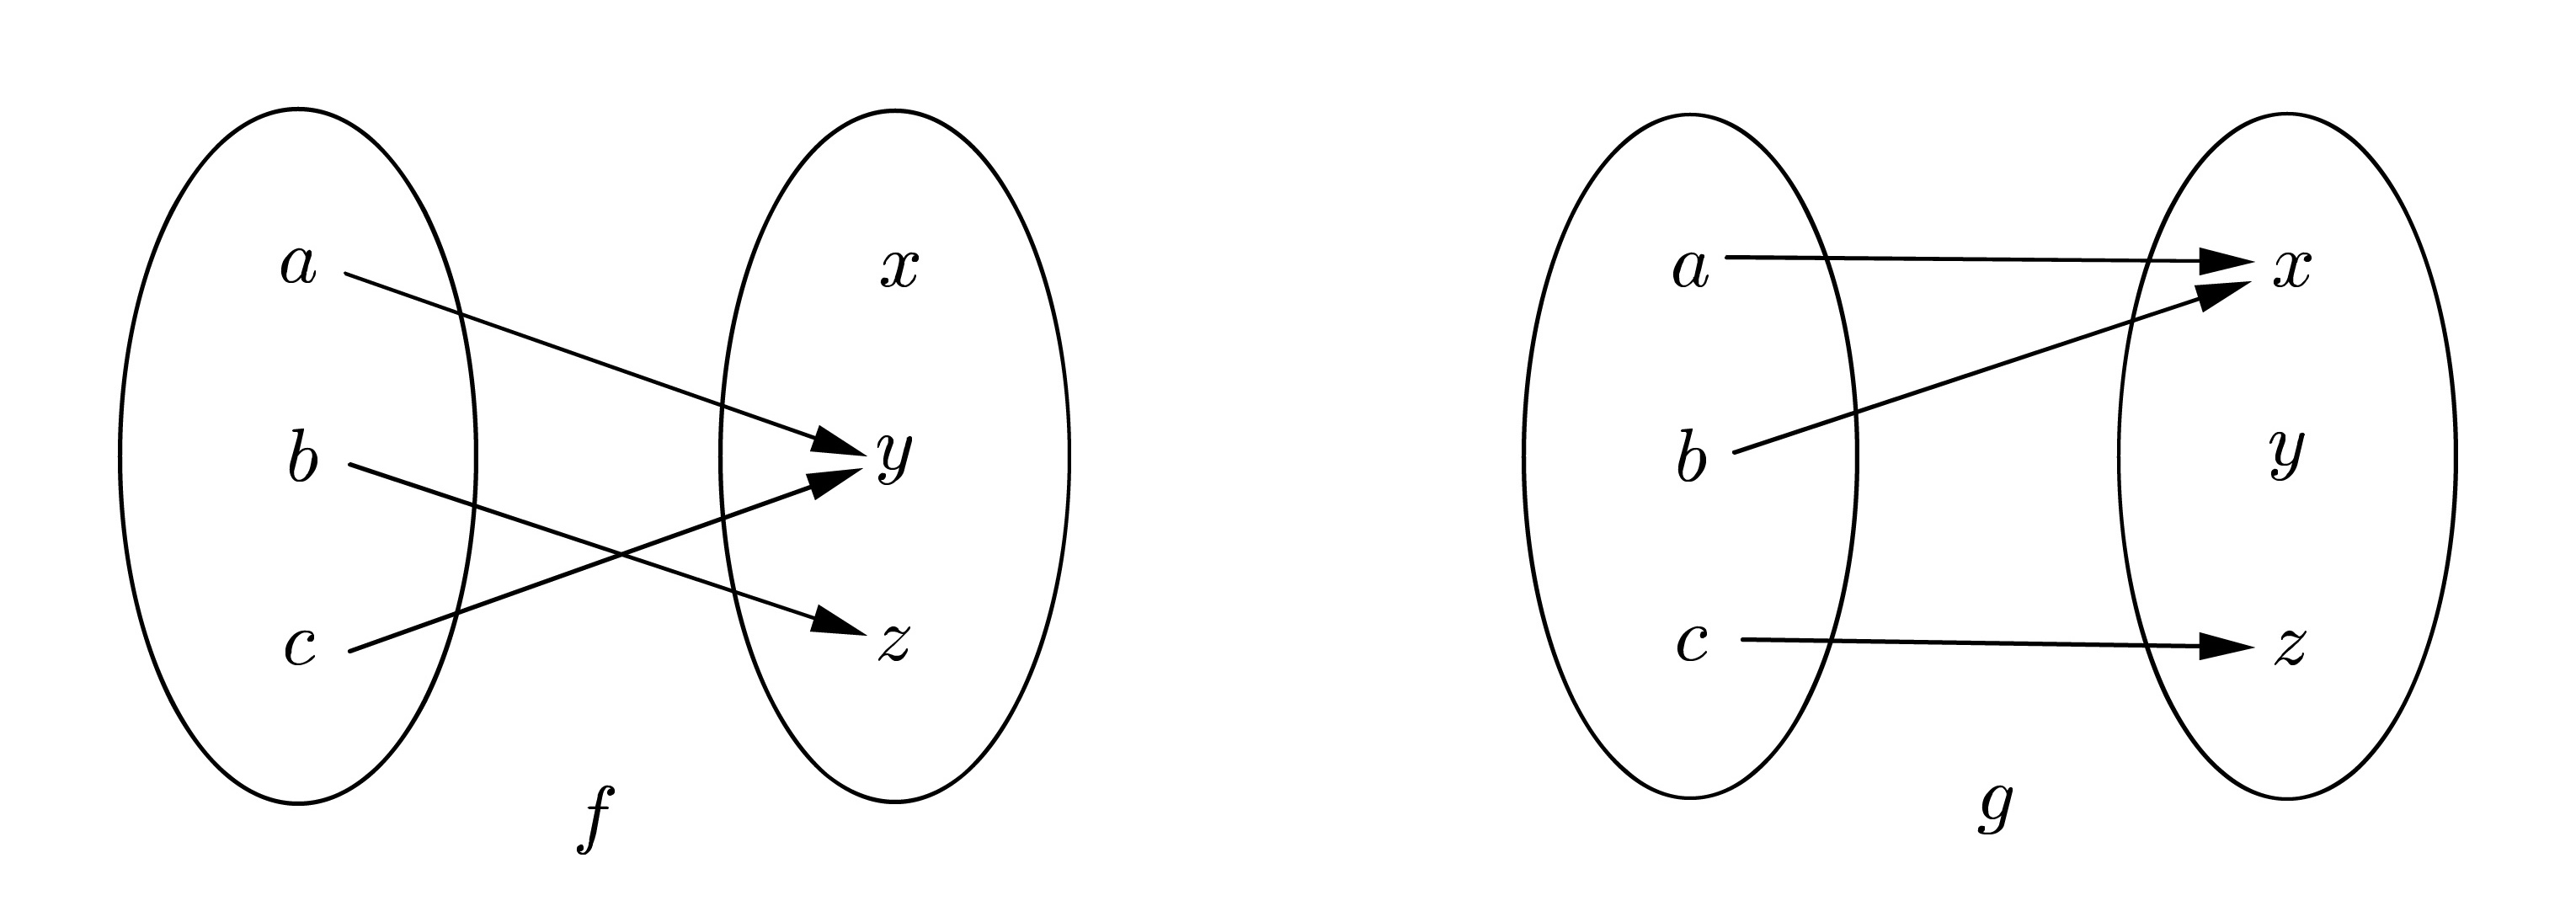
\includegraphics[width=.7\textwidth]{./images/cont1.jpg}
\end{figure}


The function $f$ is continuous since the inverse of each member of the topology $\tau^*$ on $Y$ is a member of the topology $\tau$ on $X$. The function $g$ is not continuous since $\{y,z\}\in \tau^*$ i.e. is an open subset of $Y$ but its inverse image $g^{-1}[\{y,z\}]=\{c\}$ is not an open subset of $X$ i.e. doesn't belong to $\tau$.
\end{example}

\begin{proposition}
A function $f:X \rightarrow Y$ is continuous if and only if the inverse image of every closed subset of $Y$ is a closed subset of $X$.
\end{proposition}
\begin{proof}
 Suppose $f:X\rightarrow Y$ is continuous, and $A$ a closed subset of $Y$. Then $A'$ is open, and so $f^{-1}(A')$ is open in $X$. But $f^{-1}[A']=(f^{-1}[A])'$; therefore $f^{-1}[A]$ is closed.\\
Conversely, assume $A$ closed in $Y$ implies $f^{-1}[A]$ closed in $X$. Let $G$ be an open subset of $Y$. Then $G'$ is closed in $Y$, and so $f^{-1}[G']=(f^{-1}[G])'$ is closed in $X$. Hence, $f^{-1}[G]$ is open and therefore $f$ is continuous.
\end{proof}

\begin{proposition}
Let the function $f:X\rightarrow Y$ and $g:Y\rightarrow Z$ be continuous maps. Then the composition function $g\circ f:X\rightarrow Z$ is also continuous.
\end{proposition}

\begin{proof}
Let $G$ be an open subset of $Z$. Then $g^{-1}[G]$ is open in $Y$ since $g$ is continuous. But $f$ is also a continuous, so $f^{-1}[g^{-1}[G]]$ is open in $X$. Now
$$ (g\circ f)^{-1}[G]=f^{-1}[g^{-1}[G]]$$
Thus, $(g\circ f)^{-1}[G]$ is open in $X$ for every open subset $G$ in $Z$. Therefore $g\circ f$ is a continuous map.

\end{proof}

\begin{theorem}[\textbf{The pasting lemma}]\label{pasting}
Let $X=A\cup B$, where $A$ and $B$ are closed in $X$. Let $f:A\rightarrow Y$ and $g:B\rightarrow Y$ be continuous. If $f(x)=g(x)$ for every $x\in A\cup B$, then $f$ \text{and} $g$ combine to give a continuous function $h:X\rightarrow Y$ defined by setting $h(x)=f(x)$ if $x\in A$ and $h(x)=g(x)$ if $x\in B$.
\end{theorem}
\begin{proof}
Let $C$ be a closed subset of $Y$. Now
$$h^{-1}(C)= f^{-1}(C)\cup g^{-1}(C),$$
by elementary set theory. Since $f$ is continuous, $f^{-1}(C)$ is closed in $A$ hence closed in $X$. Similarly, $g^{-1}(C)$ is closed in $B$ and therefore closed in $X$. Their union $h^{-1}(C)$ is thus closed in $X$.

\end{proof}

\section{Homeomorphism}

One major aspect of mathematics is how to find the correct notion of calling two things “equivalent.” In the theory of metric spaces\footnote{A metric on a non empty set is a function  $d: X\times X \rightarrow \mathbb{R}^+$ satisfying
\begin{enumerate}
  \item $d(x,y)\geq0$ and $d(x,x)=0$
  \item $d(x,y)=d(y,x), \forall x,y\in X$
  \item $d(x,z)\leq d(x,y)+d(y,z), \forall x,y,z\in X$
\end{enumerate}
The couple $(X,d)$ is called a metric space.}, the strongest possible such notion is called an isometry. That is, two metric spaces $X, Y$ with metrics $d_X, d_Y$ are called isometric if there exists a surjective function $f: X \to Y$ which preserves distance (i.e. $d_X(x,y) = d_Y(f(x), f(y))$ for all $x,y \in X,$ and the image $f(X)$ is all of $Y$). It is not hard to see that such functions are automatically both continuous and injective. The function $f$ is called an isometry.

Now we can call two metric spaces "the same" if they are isometric. Because we don't have distances in a topological space, the next best thing is a notion of equivalence based on continuity. This gives rise to the following definition.
\begin{definition}[\textbf{Mobius}]
Let $X$ and $Y$ be topological spaces; let $f : X\rightarrow Y$ be a bijection. If both the function $f$ and the inverse function
$$f^{-1}: Y\rightarrow X$$
are continuous, then f is called a homeomorphism.
\end{definition}

The condition that $f^{-1}$ be continuous says that for each open set $U$ of $X$, the inverse image of $U$ under the map $f^{-1}: Y\rightarrow X$ is open in $Y$ . But the inverse image of $U$ under the map $f^{-1}$ is the same as the image of $U$ under the map $f$ . So another way to define a homeomorphism is to say that it is a bijective
correspondence $f : X\rightarrow Y$ such that $f(U)$ is open if and only if $U$ is open.
 % Introduction
\clearpage  %Start a new page
\lhead{\emph{The Fundamental Group}}  % Set the left side page header to "Symbols"
\chapter{The Fundamental Group}

As we will see soon enough, the objects of the fundamental group are loops. So, we are going to make a group out of loops. A loop is nothing but a path with some base point. Now, it is a time to define a path.
\begin{definition}[\textbf{Path}]
Let $I=[0,1]$, the closed unit interval. A path from a point $a$ to a point $b$ in a topological space $X$ is a continuous function $f:I\rightarrow X$ with $f(0)=a$ and $f(1)=b$. Here $a$ and $b$ are called initial and terminal points respectively.
\end{definition}

\begin{figure}[hbt!]
\centering
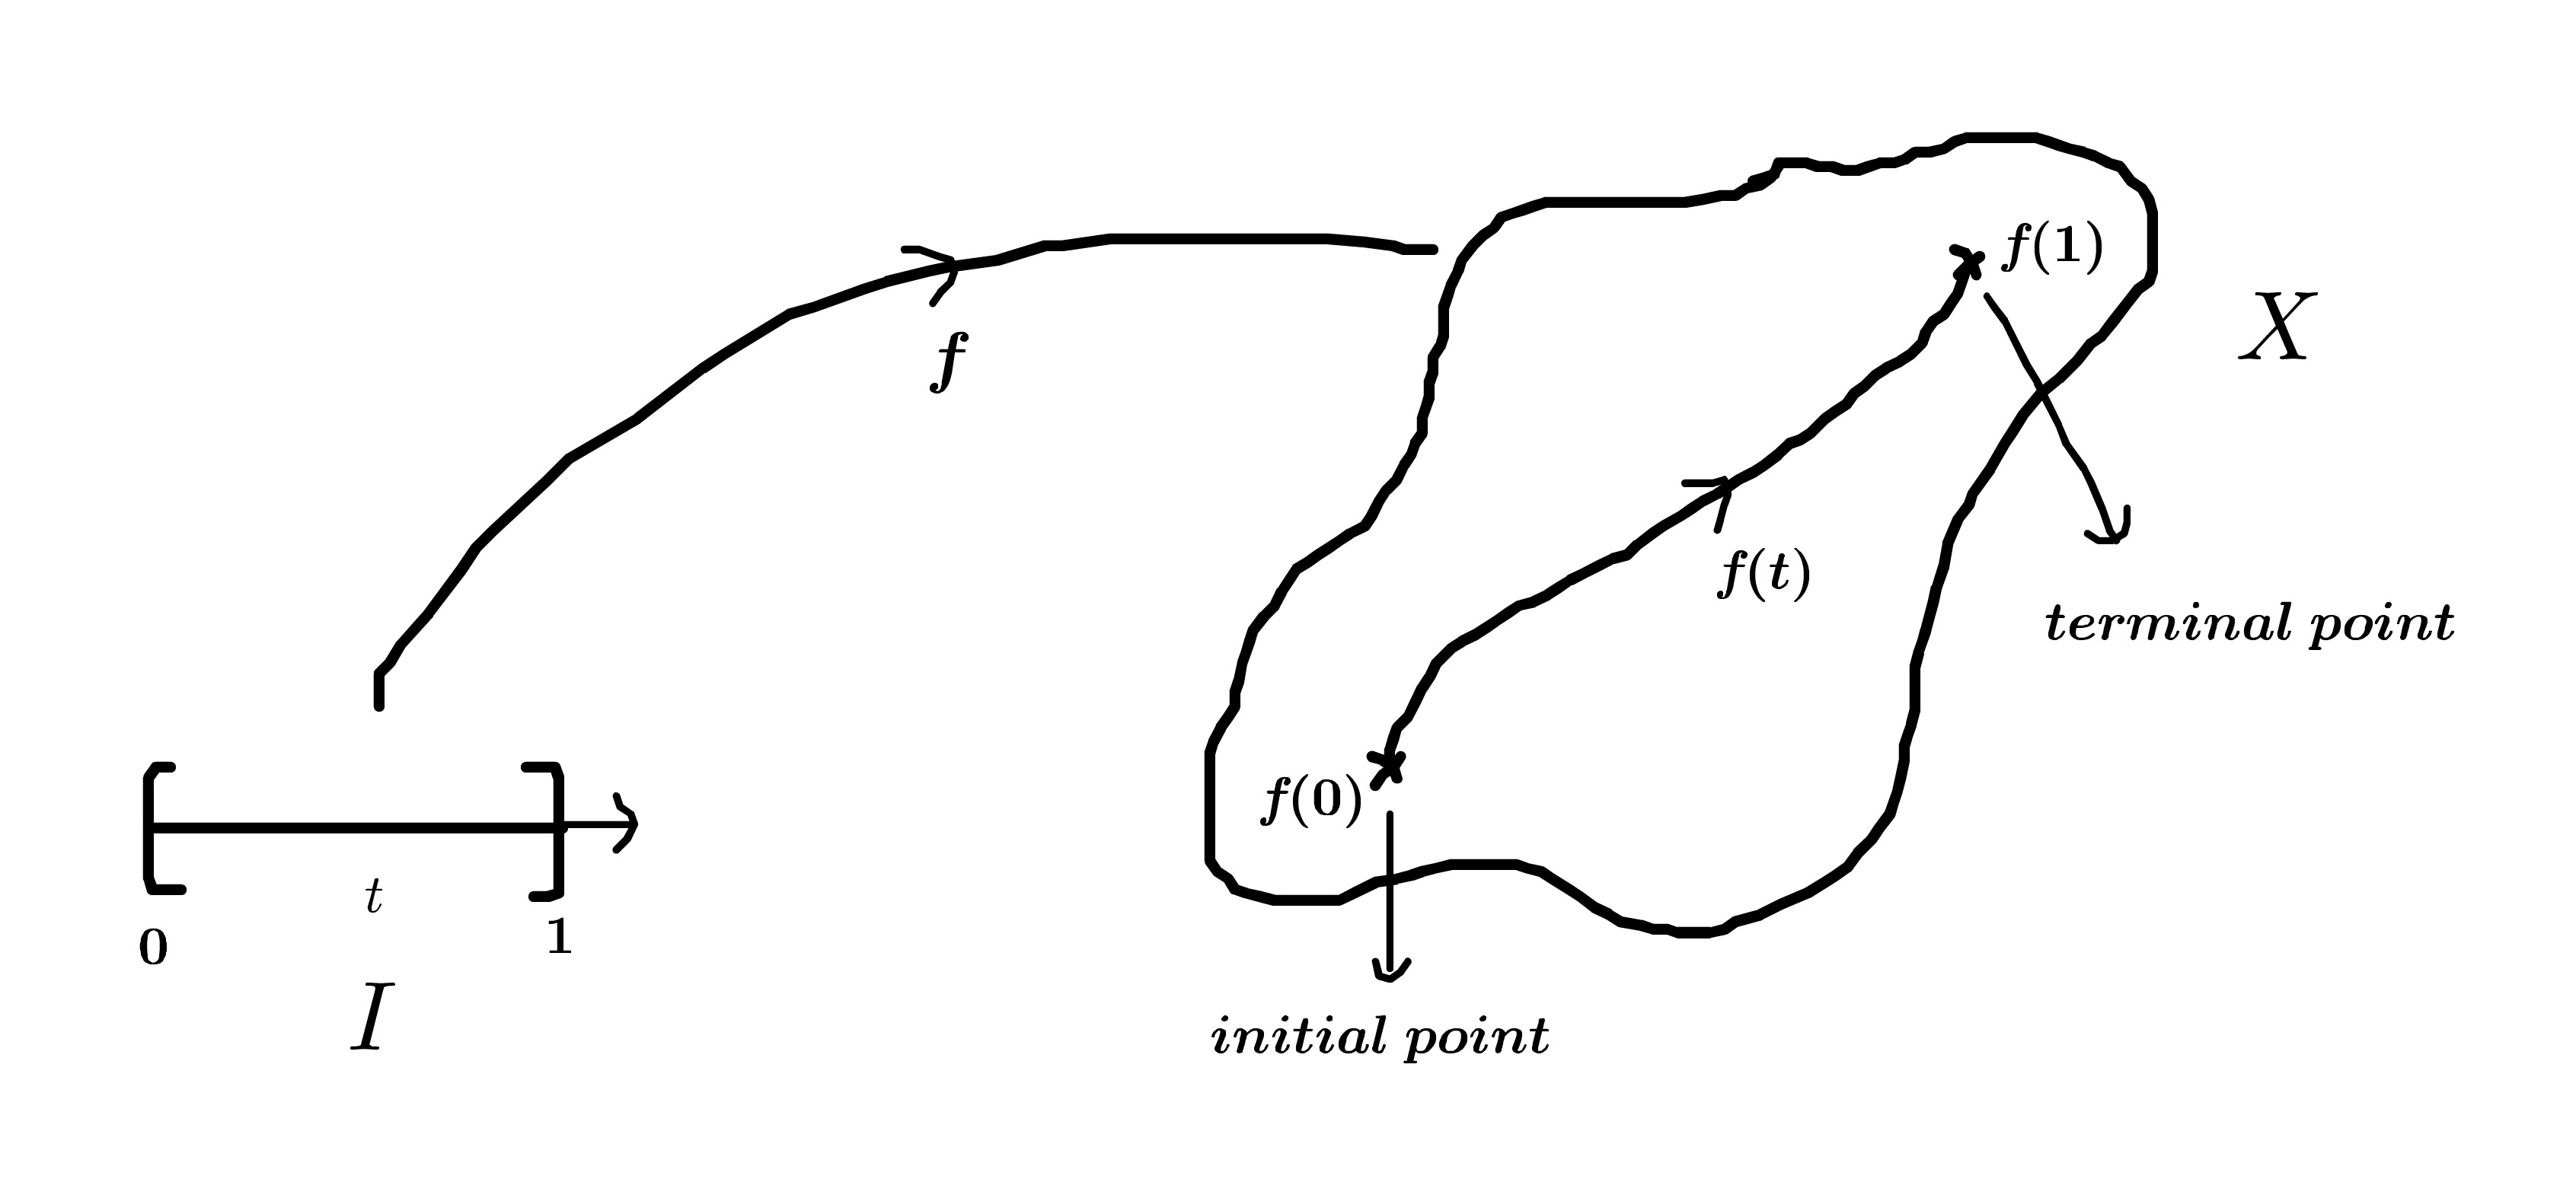
\includegraphics[width=.7\textwidth]{./images/path.jpg}
\caption{Path}
\end{figure}


\section{Homotopy}
\begin{definition}[\textbf{Homotopy}]
If $f$ and $f'$ are continuous maps of the space $X$ into the space $Y$, we say that $f$ is homotopic to $f'$ if there is a continuous map $F:X\times I \rightarrow Y$ such that
$$ F(x,0)=f(x) \qquad and \qquad F(x,1)=f'(x)$$
for each $x$. Where $I=[0,1]$ the unit interval. The map $F$ is called a \textbf{homotopy} between $f$ and $f'$. If $f$ is homotopic to $f'$ we write $f\simeq f'$. If $f\simeq f'$ and $f'$ is a constant map, we say that $f$ is \textbf{nulhomotopic}.
\end{definition}

We think of a homotopy as a continuous one-parameter family of maps from $X$ to $Y$. If we imagine the parameter $t$ as representing time, then the homotopy $F$ represents a continuous deforming of the map $f$ to the map $f'$, as $t$ goes from $0$ to $1$.

\section{Homotopy of Paths}
\begin{definition}
If $f:I\rightarrow X$ and $f':I\rightarrow X$ are two paths with the same initial point $p\in X$ and the same terminal point $q\in X$. We say that $f$ is homotopic to $f'$ if there is a continuous map $F$
$$
F: I\times I\rightarrow X \ni
$$

\begin{center}
$F(s,0)=f(s) \qquad$ and $\qquad F(s,1)=f'(s),$\\
$F(0,t)=p \qquad$ and $\qquad F(1,t)=q $
\end{center}

for each $s\in I$ and $t\in I$. We call $F$ a \textbf{path homotopy} between $f$ and $f'$ see figure \ref{path}. We denote $f\simeq_p f'$ to say $f$ is path homotopic to $f'$.
\end{definition}
\begin{figure}[hbt!]
\centering
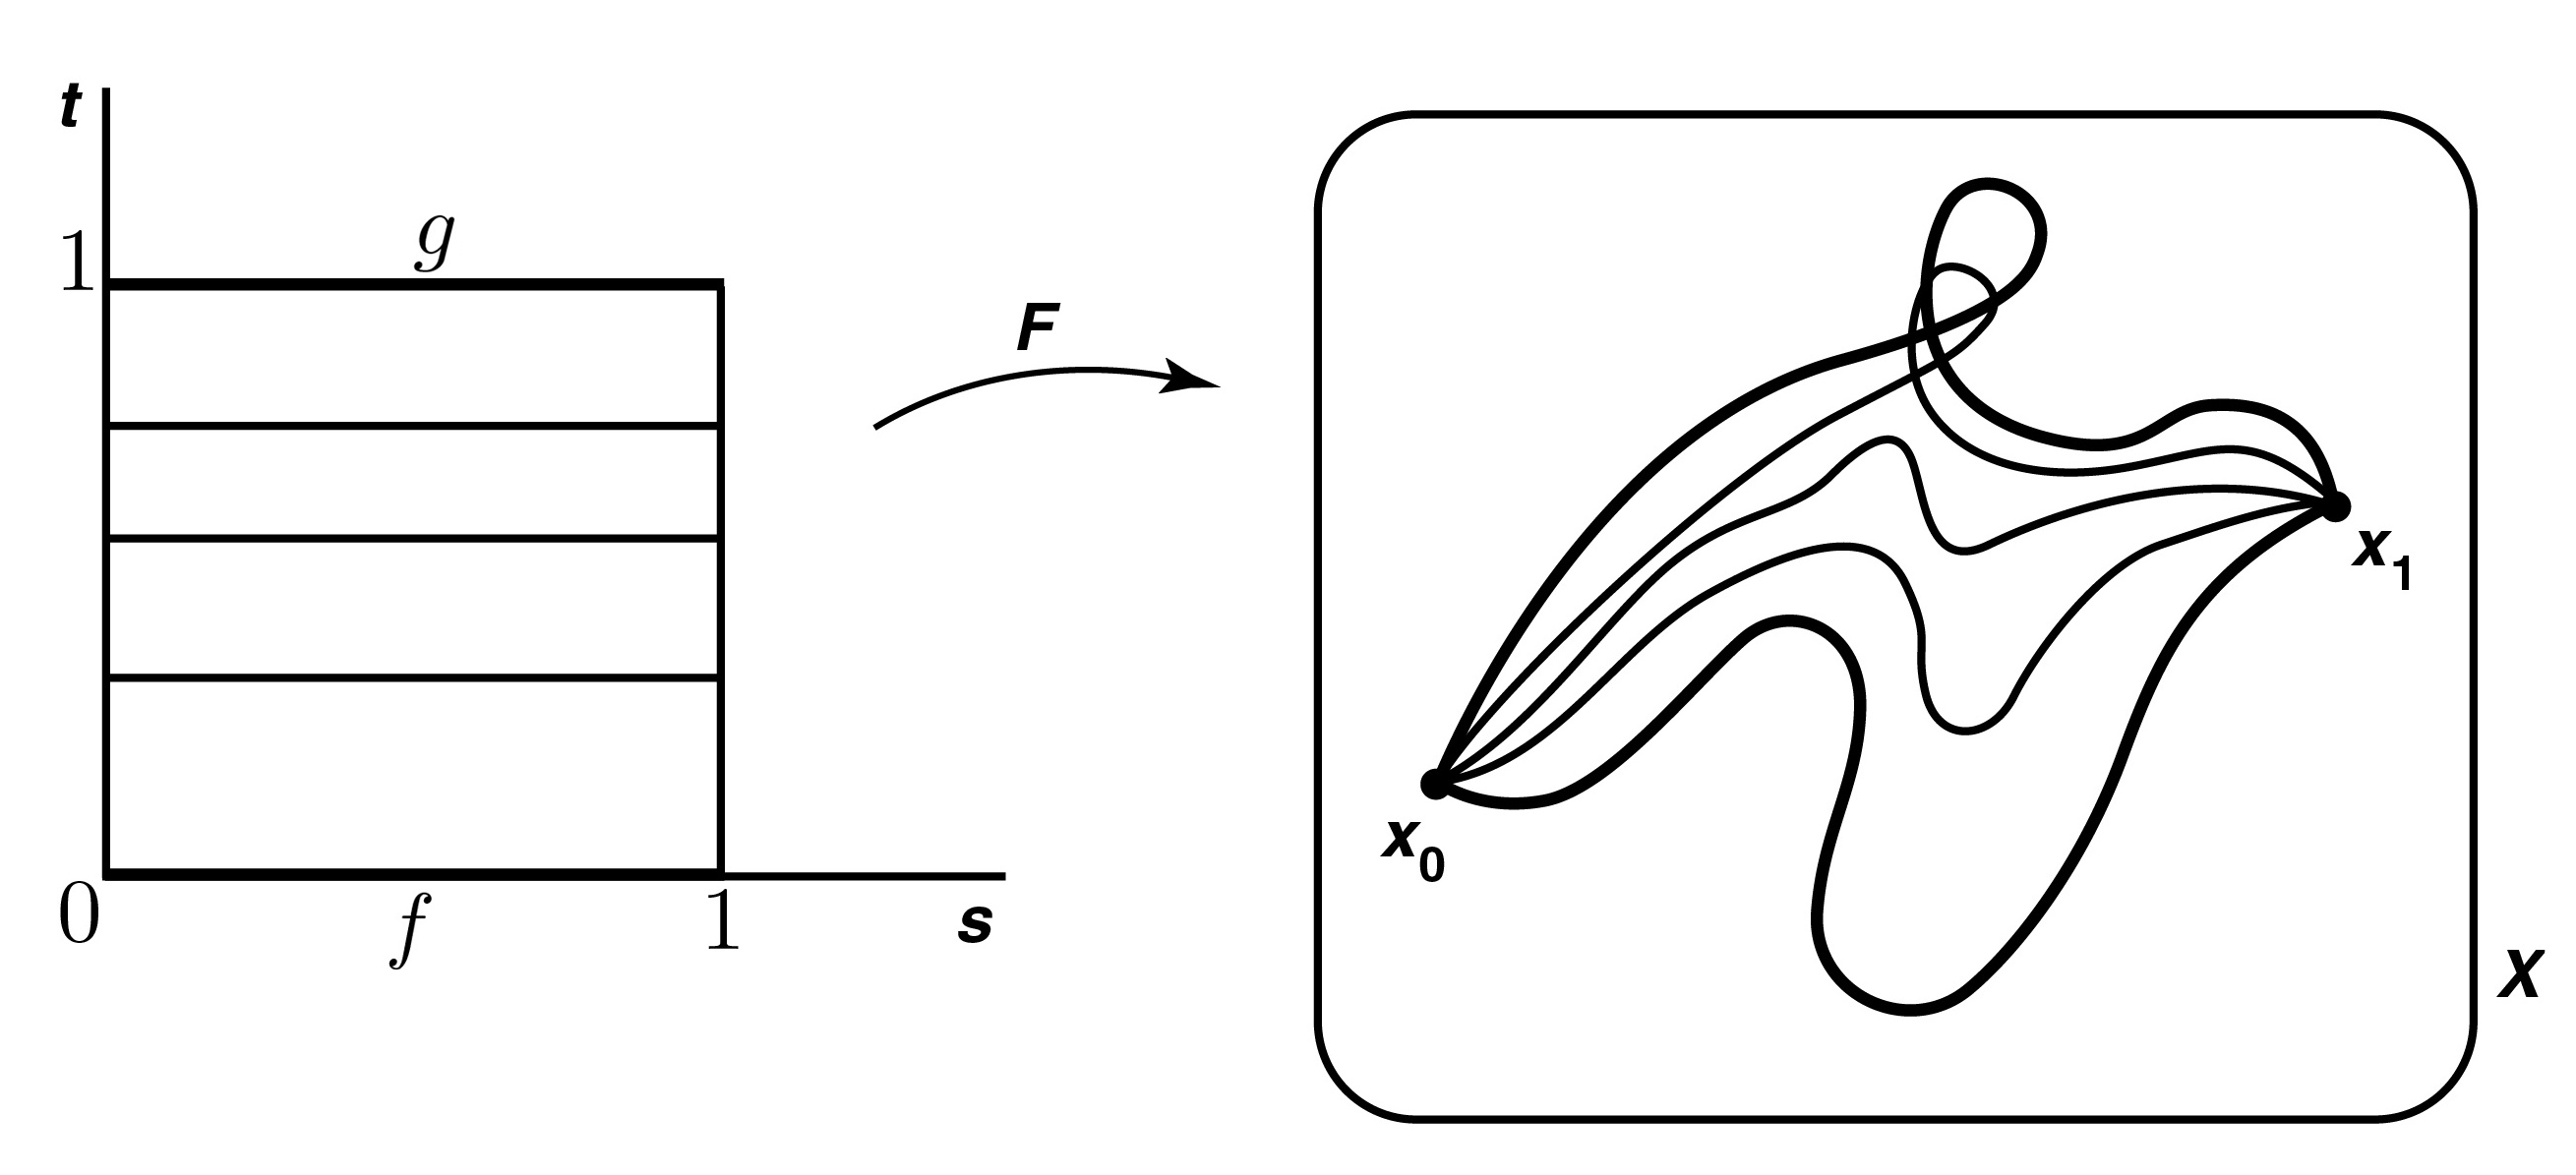
\includegraphics[width=.75\textwidth]{./images/def.jpg}
\caption{Homotopy of path}\label{path}
\end{figure}

\begin{prop}
The relations $\simeq$ and $\simeq_p$ are equivalence relations.
\end{prop}

\begin{proof}
(i) Given $f$ it is trivial that $f\simeq f$; the map $F(x,t)=f(x)$ is the required homotopy. If $f$ is a path, $F$ is a path homotopy.

(ii) Given $f\simeq f'$, we show that $f'\simeq f$. Let $F$ be a homotopy between $f$ and $f'$. Then $G(x,t)=F(x,1-t)$ is a homotopy between $f'$ and $f$. If $f$ a path homotopy  so is $G$.

(iii) Suppose that $f\simeq f'$ and $f'\simeq f''$. WTS $f\simeq f''$. Let $F$ be a homotopy between $f$ and $f''$ and let $F'$ be a homotopy between $f'$ and $f''$. Define $G:X\times I\rightarrow Y$ by the equation

$$
G(x,t)=
\begin{cases}
F(x,2t),&\mbox{ for }t\in[0,1/2]\\
F'(x,2t-1),&\mbox{ for }t\in[1/2,1]
\end{cases}
$$
The map $G$ is well-defined, since if $t=1/2$, we have
$$ F(x,2t)=f'(x)=F'(x,2t-1)$$
Because $G$ is continuous on the two closed subsets $X\times[0,1/2]$ and $X\times[1/2,1]$ of $X\times I$, it is continuous on all of $X\times I$, by pasting lemma (\ref{pasting}). Thus $G$ is the required homotopy between $f$ and $f"$.
\end{proof}
\medskip
The following figure illustrates if $F$ and $F'$ are path homotopies, so is $G$
\begin{figure}[hbt!]
\centering
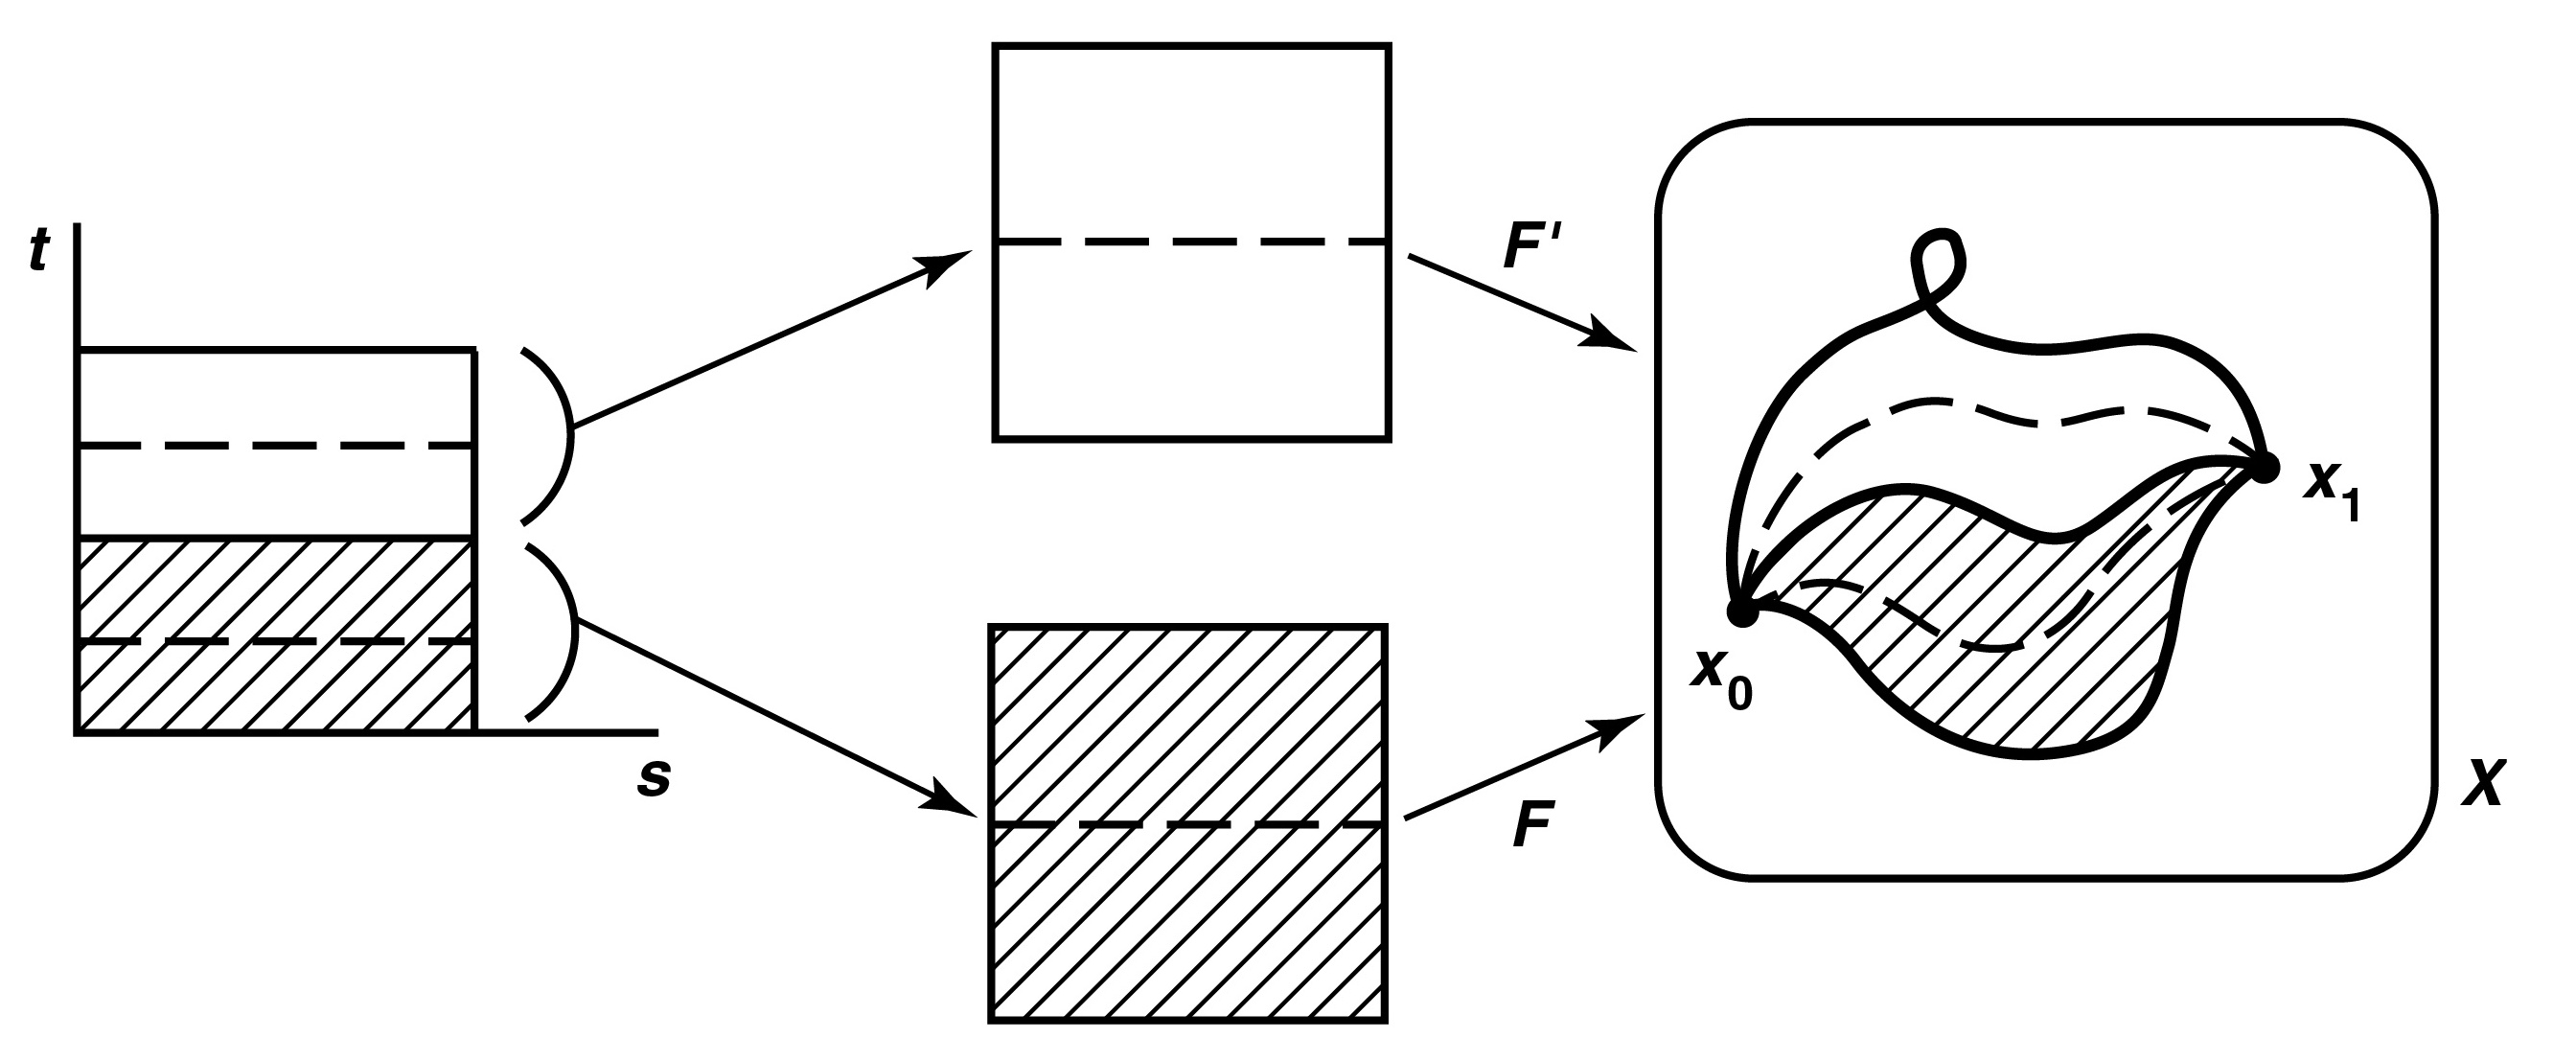
\includegraphics[width=.8\textwidth]{./images/equiv.jpg}
\caption{Transitive property of the homotopy}
\end{figure}


\begin{example}
Let $f$ and $g$ be any two continuous maps of space $X$ into $\mathbb{R}^2$ It is easy to see that $f$ and $g$ are homotopic; the map
$$
F(x,t)=(1-t)f(x)+tg(x)
$$
is a homotopy between them. It is called a straight-line homotopy because it moves the point $f(x)$ to the point $g(x)$ along the straight-line segment joining them.
\end{example}
\begin{prop}\label{homocomp}
If $h, h'$ are homotopic maps from $X$ into $Y$ and $k, k'$ are homotopic maps from $Y$ into $Z$ , then $k\circ h \simeq k' \circ h'$.
\end{prop}


\begin{proof}
Since $h\simeq h'$ there is a homotopy $H:X\times I \rightarrow Y$ with $H(s,0)=h(s),$ $H(s,1)=h'(s).$
Since $k\simeq k'$ there is a homotopy $K:Y\times I \rightarrow Z$ with $K(s,0)=k(s),$ $K(s,1)=kh'(s).$ Then define $F: X\times I\rightarrow Z$ by

$$
F(s,t)=
\begin{cases}
k(H(s,2t)),&0\leq t\leq 1/2\\
K(h'(s),2t-1),&1/2\leq t\leq 1
\end{cases}
$$
Then let's check that $F$ does what it ought to do, at different values of $t$.\\
\begin{align*}
t=0,\qquad F(s,o)=k(H(s,o))=k(h(s))=k\circ h(s)\\
t=1/2,\qquad F(s,1/2)=k(H(s,1))=k(h'(s))=k\circ h'(s)\\
\qquad \qquad F(s,1/2)=K(h'(s),0))=k(h'(s))=k\circ h'(s)\\
t=1,\qquad F(s,1)=K(h'(s),1)=k'(h'(s))=k'\circ h'(s)
\end{align*}
Thus $F$ is the desired homotopy.
\end{proof}


\begin{definition}
A constant path in a topological space $Y$ is a constant function from $I$ into $Y$. i.e. $f:I\rightarrow Y$ is a constant path if there is $y_0\in Y$ such that $f(s)=y_0$ for all $s\in I$.
\end{definition}

\begin{definition}
Two topological spaces $X$ $\&$ $Y$ are said to be homotopy equivalent or of the \textbf{same same homotopy} type if there exist a continuous maps $f:X\rightarrow Y$ and $g:Y\rightarrow X$ such that $g\circ f $ is homotopic to the identity map $id_X$ and $f\circ g\simeq id_Y$.
\end{definition}




Homeomorphic spaces are of the same homotopy type. To show this let $X$ and $Y$ be homeomorphic spaces. Then there exists a continuous map $f:X\rightarrow Y$ with a continuous inverse $f^{-1}:Y\rightarrow X$. Thus $f\circ f^{-1}=id_Y$ and $f^{-1}\circ f=id_X$. Since homotopy is an equivalence relation this implies $f\circ f^{-1}\simeq id_Y$ and $f^{-1}\circ f\simeq id_X$  Q.E.D. But the converse is not true: for example, a solid disk is not homeomorphic to a single point (since there is no bijection between them), although the disk and the point are homotopy equivalent (since you can deform the disk along radial lines continuously to a single point). Spaces that are homotopy equivalent to a point are called contractible.

\begin{prop}
Same homotopy type is an equivalence relation on the collection of topological space.
\end{prop}

\begin{proof}
\begin{description}
  \item[Reflexive:] Let $X$ be a topological space. Define $id:X\rightarrow X$ by $id(x)=x.$
  \item[Symmetric:] Let $X $ and $Y$ are spaces of the same homotopy. Then there exist a continuous maps $f:X\rightarrow Y$ and $g:Y\rightarrow X$ such that $g\circ f $ is homotopic to the identity map $id_X$ and $f\circ g\simeq id_Y$. Thus $Y$ and $X$ are of the same homotopy.
  \item[Transitive:] Suppose $X $ and $Y$ are spaces of the same homotopy. Then there exist a continuous maps $f_1:X\rightarrow Y$ and $g_1:Y\rightarrow X$ such that $g_1\circ f_1 \simeq id_X$ and $f_1\circ g_1\simeq id_Y$. Similarly, if $Y $ and $Z$ are spaces of the same homotopy, then there exist a continuous maps $f_2:Y\rightarrow Z$ and $g_2:Z\rightarrow Y$ such that $g_2\circ f_2 \simeq id_Y$ and $f_2\circ g_2\simeq id_Z$. WTS $(g_1\circ g_2)\circ(f_2\circ f_1)\simeq id_X$ and $(f_2\circ f_1)\circ(g_1\circ g_2)\simeq id_Z$. Now
   $$(g_1\circ g_2)\circ(f_2\circ f_1)=g_1\circ \underbrace{(g_2\circ f_2)\circ f_1 \simeq g_1\circ (id_Y)}_{\Delta_1}\circ f_1= g_1\circ f_1\simeq id_X.$$
Similarly, $$(f_2\circ f_1)\circ(g_1\circ g_2)=f_2\circ \underbrace{(f_1\circ g_1)\circ g_2 \simeq f_2\circ (id_Y)}_{\Delta_2}\circ g_2= f_2\circ g_2\simeq id_Z.$$
\end{description}
The steps $\Delta_1$ and $\Delta_2$ are actually true by proposition (\ref{homocomp}).
\end{proof}

\medskip
\begin{definition}[\textbf{Concatenation}]
If $f$ is a path in $X$ from $x_0$ to $x_1$, and if $g$ is a path from $x_1$ to $x_2$, we define the \textbf{product} of $f\ast g$ of $f$ and $g$ to be the path $h$ given by the equations
$$
h(s)=
\begin{cases}
f(2s),&\mbox{ for }s\in[0,1/2]\\
g(2s-1),&\mbox{ for }s\in[1/2,1]
\end{cases}
$$
\end{definition}
The function $h$ is well-defined and continuous, by the pasting lemma (\ref{pasting}); it is a path in $X$ from $x_0$ to $x_2$. We think of $h$ as the path whose first half is the path $f$ and whose second half is the path $g$.
The product operation on paths induces a well-defined operation on path-homotopy classes, defined by the equation
$$[ f ] \ast [g] = [ f \ast g].$$
To verify this fact, let $F$ be a path homotopy between $f$ and $f'$ and let $G$ be a path homotopy between $g$ and $g'$. Define
$$
H(s,t)=
\begin{cases}
F(2s,t),&\mbox{ for }s\in[0,1/2]\\
G(2s-1,t),&\mbox{ for }s\in[1/2,1]
\end{cases}
$$
Because $F(1, t) = x_1 = G(0, t)$ for all $t$, the map $H$ is well-defined; it is continuous by the pasting lemma (\ref{pasting}).


\section{The Fundamental Group}

\begin{definition}
A loop in a topological space is a path in the space whose initial point and terminal point are the same. If the initial point and terminal point of a loop in the topological space $X$ are both the point $x_0\in X$, we will say that the loop is based at $x_0$.
\end{definition}

Let $X$ be a topological space and $x_0$ be a point in $X$. Then the $x_0$ neighborhood of curves in $X$, $C(X,x_0)$, is the collection of all continuous mappings $f:I\rightarrow X$ of the unit interval into $X$ such that $f(0)=x_0=f(1)$. i.e. the collection of all loops based at $x_0$.


\begin{definition}
Let $f$ and $g$ be two maps in $C(X,x_0)$ that means $f$ and $g$ are loops based at $x_0$. Then $f$ is homotopic to $g~modulo~x_0$ if $f$ and $g$ are homotopic in a usual sense with some additional restriction. Here is the restriction: If H is the homotopy between $f$ and $g$ , then $H(0,t)=x_0=H(1,t)$.
\end{definition}

\begin{theorem}
The set of path homotopy equivalence class of loops based at $x_0\in X$ is a group under the ''multiplication'' defined by $[\alpha][\beta]=[\alpha\beta]$. This group is denoted by $\pi_1(X,x_0)$ and is called the fundamental group of $X$ at $x_0$.
\end{theorem}
\begin{proof}
WTS that the four group axioms are satisfied here.
\begin{description}
  \item[I.] Our first task is to show the ''multiplication'' is well-defined. Thus we have to show that it is independent of what representatives $\alpha$ and $\beta$ of $[\alpha]$ and $[\beta]$ are used. This done by proving if $\alpha_1\simeq \alpha_2$ ,$\beta_1\simeq\beta_2$ then $\alpha_1\beta_1\simeq\alpha_2\beta_2$. To show this let $H_1$ and $H_2$ be homotopies such that
      $$ H_1(s,0)=\alpha_1(s), H_1(s,1)=\alpha_2(s), \qquad H_1(0,t)=x_0=H_1(1,t)$$
      $$ H_2(s,0)=\beta_1(s), H_2(s,1)=\beta_2(s), \qquad H_2(0,t)=x_0=H_2(1,t)$$
  Define
$$
H(s,t)=
\begin{cases}
H_1(2s,t),&\mbox{ for }s\in[0,1/2]\\
H_2(2s-1,t),&\mbox{ for }s\in[1/2,1]
\end{cases}
$$
The mapping $H$ is well-defined and it is continuous by pasting lemma. Also
\[
    H(s,0) = \left\{\begin{array}{lr}
        H_1(2s,0)=\alpha_1(2s), & \text{ for }\ 0\leq s\leq 1/2\\
        H_2(2s-1,0)=\beta_1(2s-1), & \text{ for }\ 1/2\leq s\leq 1
        \end{array}\right\} = (\alpha_1\ast\beta_1)(s)
\]
and
\[
    H(s,1) = \left\{\begin{array}{lr}
        H_1(2s,1)=\alpha_2(2s), & \text{ for }\ 0\leq s\leq 1/2\\
        H_2(2s-1,1)=\beta_2(2s-1), & \text{ for }\ 1/2\leq s\leq 1
        \end{array}\right\} = (\alpha_2\ast\beta_2)(s)
\]
Thus $\pi_1(X,x_0)$ is closed under this operation.
  \item[II.] The associative property follows if we can show that $(\alpha \ast \beta)\ast\gamma \simeq\alpha(\beta\ast\gamma)$

  From the definition
$$
[(\alpha\ast\beta)\ast\gamma](s)=
\begin{cases}
\alpha(4s),&\mbox{ for }\ 0\leq s\leq 1/4\\
\beta(4s-1),&\mbox{ for }\ 1/4\leq s\leq 1/2\\
\gamma(2s-1)&\mbox{ for }\ 1/2\leq s\leq 1\\
\end{cases}
$$
and
$$
[\alpha\ast(\beta\ast\gamma)](s)=
\begin{cases}
\alpha(2s),&\mbox{ for }\ 0\leq s\leq 1/2\\
\beta(4s-2),&\mbox{ for }\ 1/2\leq s\leq 3/4\\
\gamma(4s-3)&\mbox{ for }\ 3/4\leq s\leq 1\\
\end{cases}
$$
A homotopy $H$ between these two mappings may be given as follows
$$
H(s,t)=
\begin{cases}
\alpha(\frac{4s}{t+1}),&\mbox{ for }\ t\geq 4s-1\\
\beta(4s-t-1),&\mbox{ for }\ 4s-1\geq t\geq 4s-2\\
\gamma(\frac{4s-t-2}{2-t})&\mbox{ for }\ 4s-2\geq t\\
\end{cases}
$$
We can use the following diagram to obtain the above homotopy

\begin{figure}[hbt!]
\centering
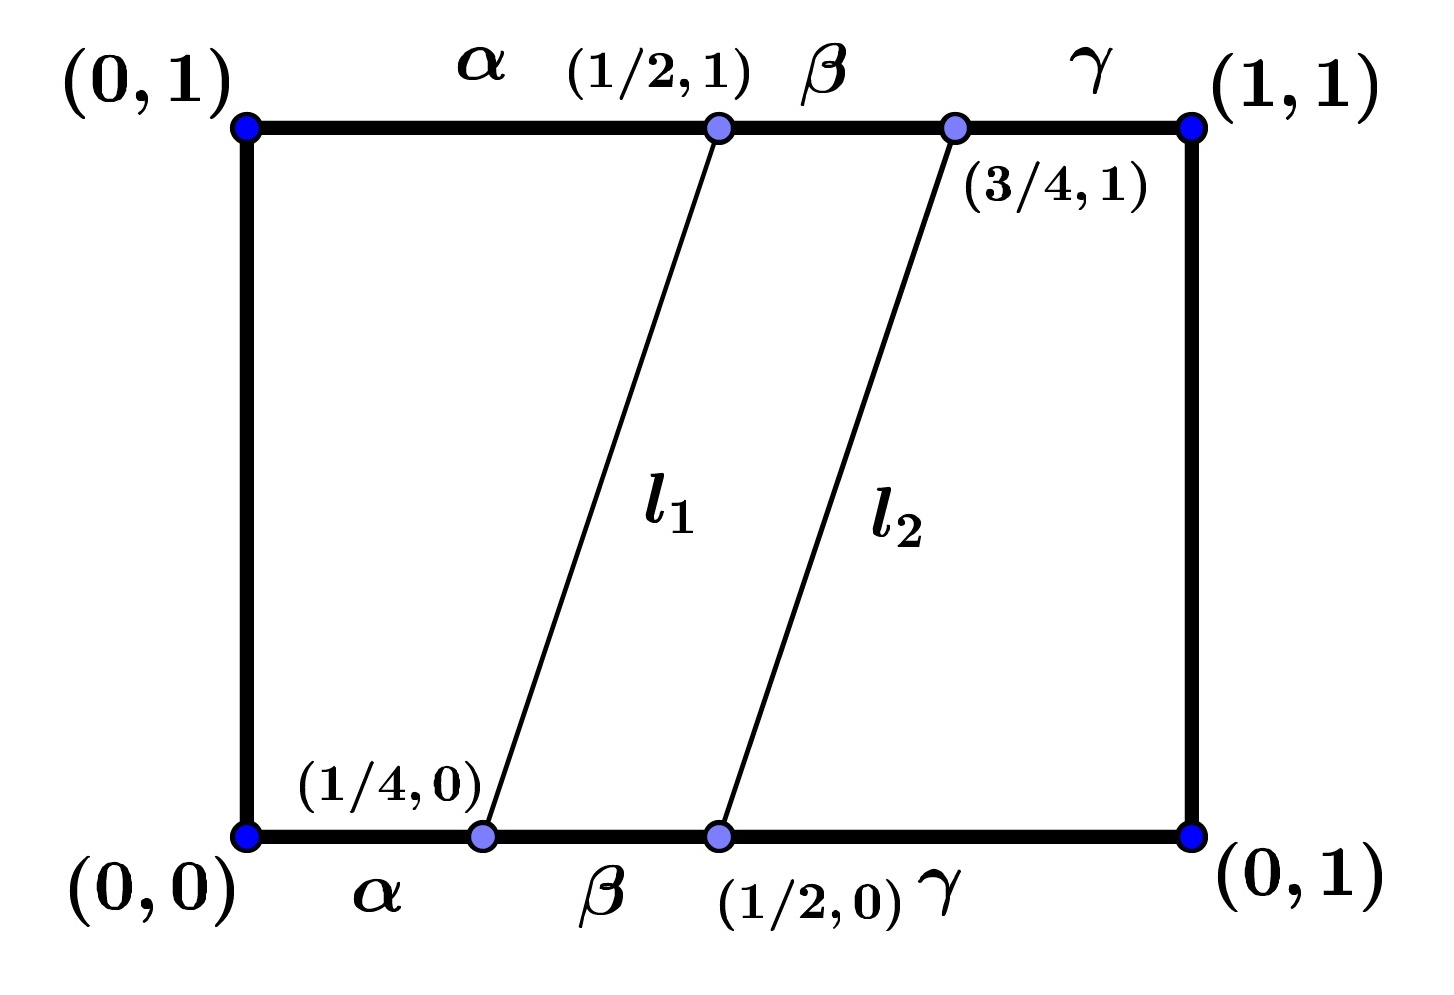
\includegraphics[width=.6\textwidth]{./images/Asso.jpg}
\caption{Associativity property}
\end{figure}

To check that $H$ is the desired homotopy

\[
H(s,0)=\left\{\begin{array}{lr}
\alpha(4s),&\text{for}\ 0\geq 4s-1 \text{ or } 0\leq s\leq1/4 \\
\beta(4s-1),&\mbox{ for }\ 4s-1\geq 0\geq 4s-2 \text{ or } 1/4\leq s\leq1/2\\
\gamma(2s-1)&\mbox{ for }\ 4s-2\geq 0 \text{ or } 1/2\leq s\leq1
\end{array}\right\}=(\alpha\ast\beta)\ast\gamma
\]

and

\[
H(s,1)=\left\{\begin{array}{lr}
\alpha(2s),&\text{for}\ 1\geq 4s-1 \text{ or } 0\leq s\leq1/2\\
\beta(4s-2),&\mbox{ for }\ 4s-1\geq 1\geq 4s-2 \text{ or } 1/2\leq s\leq 3/4\\
\gamma(4s-3)&\mbox{ for }\ 4s-2\geq 1 \text{ or } 3/4\leq s\leq 1
\end{array}\right\}=\alpha\ast(\beta\ast\gamma)
\]
Hence associativity.
  \item[III.] The existence of an identity.

Let $e_{x_0}$ denote the constant mapping $e_{x_0}(x)=x_0$ for all $x\in I$. We claim the equivalence class $[e_{x_0}]$ is the identity element of $\pi_1(X,x_0)$. To prove this it suffices to show that $\alpha\ast e_{x_0}$ for any function in $C(X,x_0)$. This is done by constructing the homotopy
$$
H(s,t)=
\begin{cases}
\alpha(\frac{2s}{1+t}),&\mbox{ for }\ t\geq 2s-1\\
x_0,&\mbox{ for }\  t\leq 2s-1
\end{cases}
$$
The continuity of $H$ is in question where $t=2s-1$, but for any such point $H(s,t)=x_0$, so $H$ is continuous as required. A check at the boundary conditions shows that
\[ H(s,0) = \left\{\begin{array}{lr}
        \alpha(2s) & \text{ for }\ 0\ge 2s-1 \text{ or } 0\leq s\leq 1/2 \\
        x_0 & \text{ for }\ 0\leq 2s-1 \text{ or } 1/2\leq s\leq 1
        \end{array}\right\} = \alpha\ast e_{x_0}
\]
and $H(s,1)=\alpha(s) \text{ for } 1\ge 2s-1 \text{ or } 0\leq s\leq 1.$
  \item[IV.] The existence of inverse element.

  To show this let $\alpha$ be any mapping in $C(X,x_0)$ and define a new mapping $\alpha^{-1}$ by setting
  $$\alpha^{-1}(s)=\alpha(1-s)$$
  Thus, $\alpha^{-1}(0)=\alpha(1)=\alpha^{-1}(1)=\alpha(0),$ so $\alpha^{-1}$ is an element of $C(X,x_0)$. We want to show $\alpha\ast\alpha^{-1}\simeq e_{x_0}$. By definition
$$
(\alpha\ast\alpha^{-1})(s)=
\begin{cases}
\alpha(2s),&\mbox{ for }\ 0\leq s\leq 1/2\\
\alpha^{-1}(2s-1)=\alpha(2-2s),&\mbox{ for }\  1/2\leq s\leq1
\end{cases}
$$
Now, we construct a homotopy between $\alpha\ast\alpha^{-1}$ and $e_{x_0}$ by setting
$$
H(s,t)=
\begin{cases}
\alpha(\frac{2s}{1-t}), & \text{for }t\geq 2s-1, 0\leq s\leq 1/2\\
        x_0,  & \text{for } t\geq 1-2s, 0\leq s\leq 1/2 ;\\
                               & t\geq 2s-1, 1/2\leq s\leq 1\\
       \alpha(\frac{2s-2}{t-1}), & \text{for } t\leq 2s-1, 1/2\leq s \leq 1
\end{cases}
$$
To check the continuity of $H$, at $t=1-2s$
$$ H(s,t)=\alpha\biggl(\frac{2s}{1-(1-2s)}\biggl)=\alpha(1)=x_0$$
And for $t=2s-1$
$$ H(s,t)=\alpha\biggl(\frac{2s-2}{2s-1-1}\biggl)=\alpha(1)=x_0$$
Hence $H$ has the necessary continuity. Checking the boundary conditions
\[ H(s,0) = \left\{\begin{array}{lr}
        \alpha(2s) & \text{ for }\ 0\leq 1-2s \text{ or } 0\leq s\leq 1/2 \\
        x_0 & \text{ for }\ 2s-1\leq0\leq1-2s \text{ or }  s\leq 1/2\\
        \alpha(\frac{2s-2}{-1})=\alpha(2-2s) & \text{ for }\ 0\leq 2s-1 \text{ or } 1/2\leq s\leq 1
        \end{array}\right\} = \alpha\ast \alpha^{-1}
\]
And $H(s,1)=x_0=e_{x_0}$
This shows that the class $[f^{-1}]$ is the inverse of $[f]$.
\end{description}
This completes the proof that $\pi_1(X,x_0)$ is a group, the fundamental group of $X$ based at $x_0$.
\end{proof}

Instead of the fundamental group of $X$ based at $x_0$ it would be nice to have the fundamental group of $X$. In other words, we would like to have the fundamental group depend only on the space, and not on the particular point of the space that we base our loops at.

\medskip
\begin{thm}

Let $x_0,x_1\in X$. If there is a path in $X$ from $x_0$ to $x_1$ then the groups $\pi_1(X,x_0)$ and $\pi_1(X,x_1)$ are isomorphic.

\end{thm}

\begin{proof}
To show the two groups are isomorphic is just a matter of finding a bijective map from one to the other.

Let $\gamma$ be a path from $x_0$ to $x_1$. If $\alpha$ is a loop based at $x_0$, then $(\gamma^{-1}\ast\alpha)\ast \gamma $ is a closed path based at $x_1$.

\begin{figure}[hbt!]
\centering
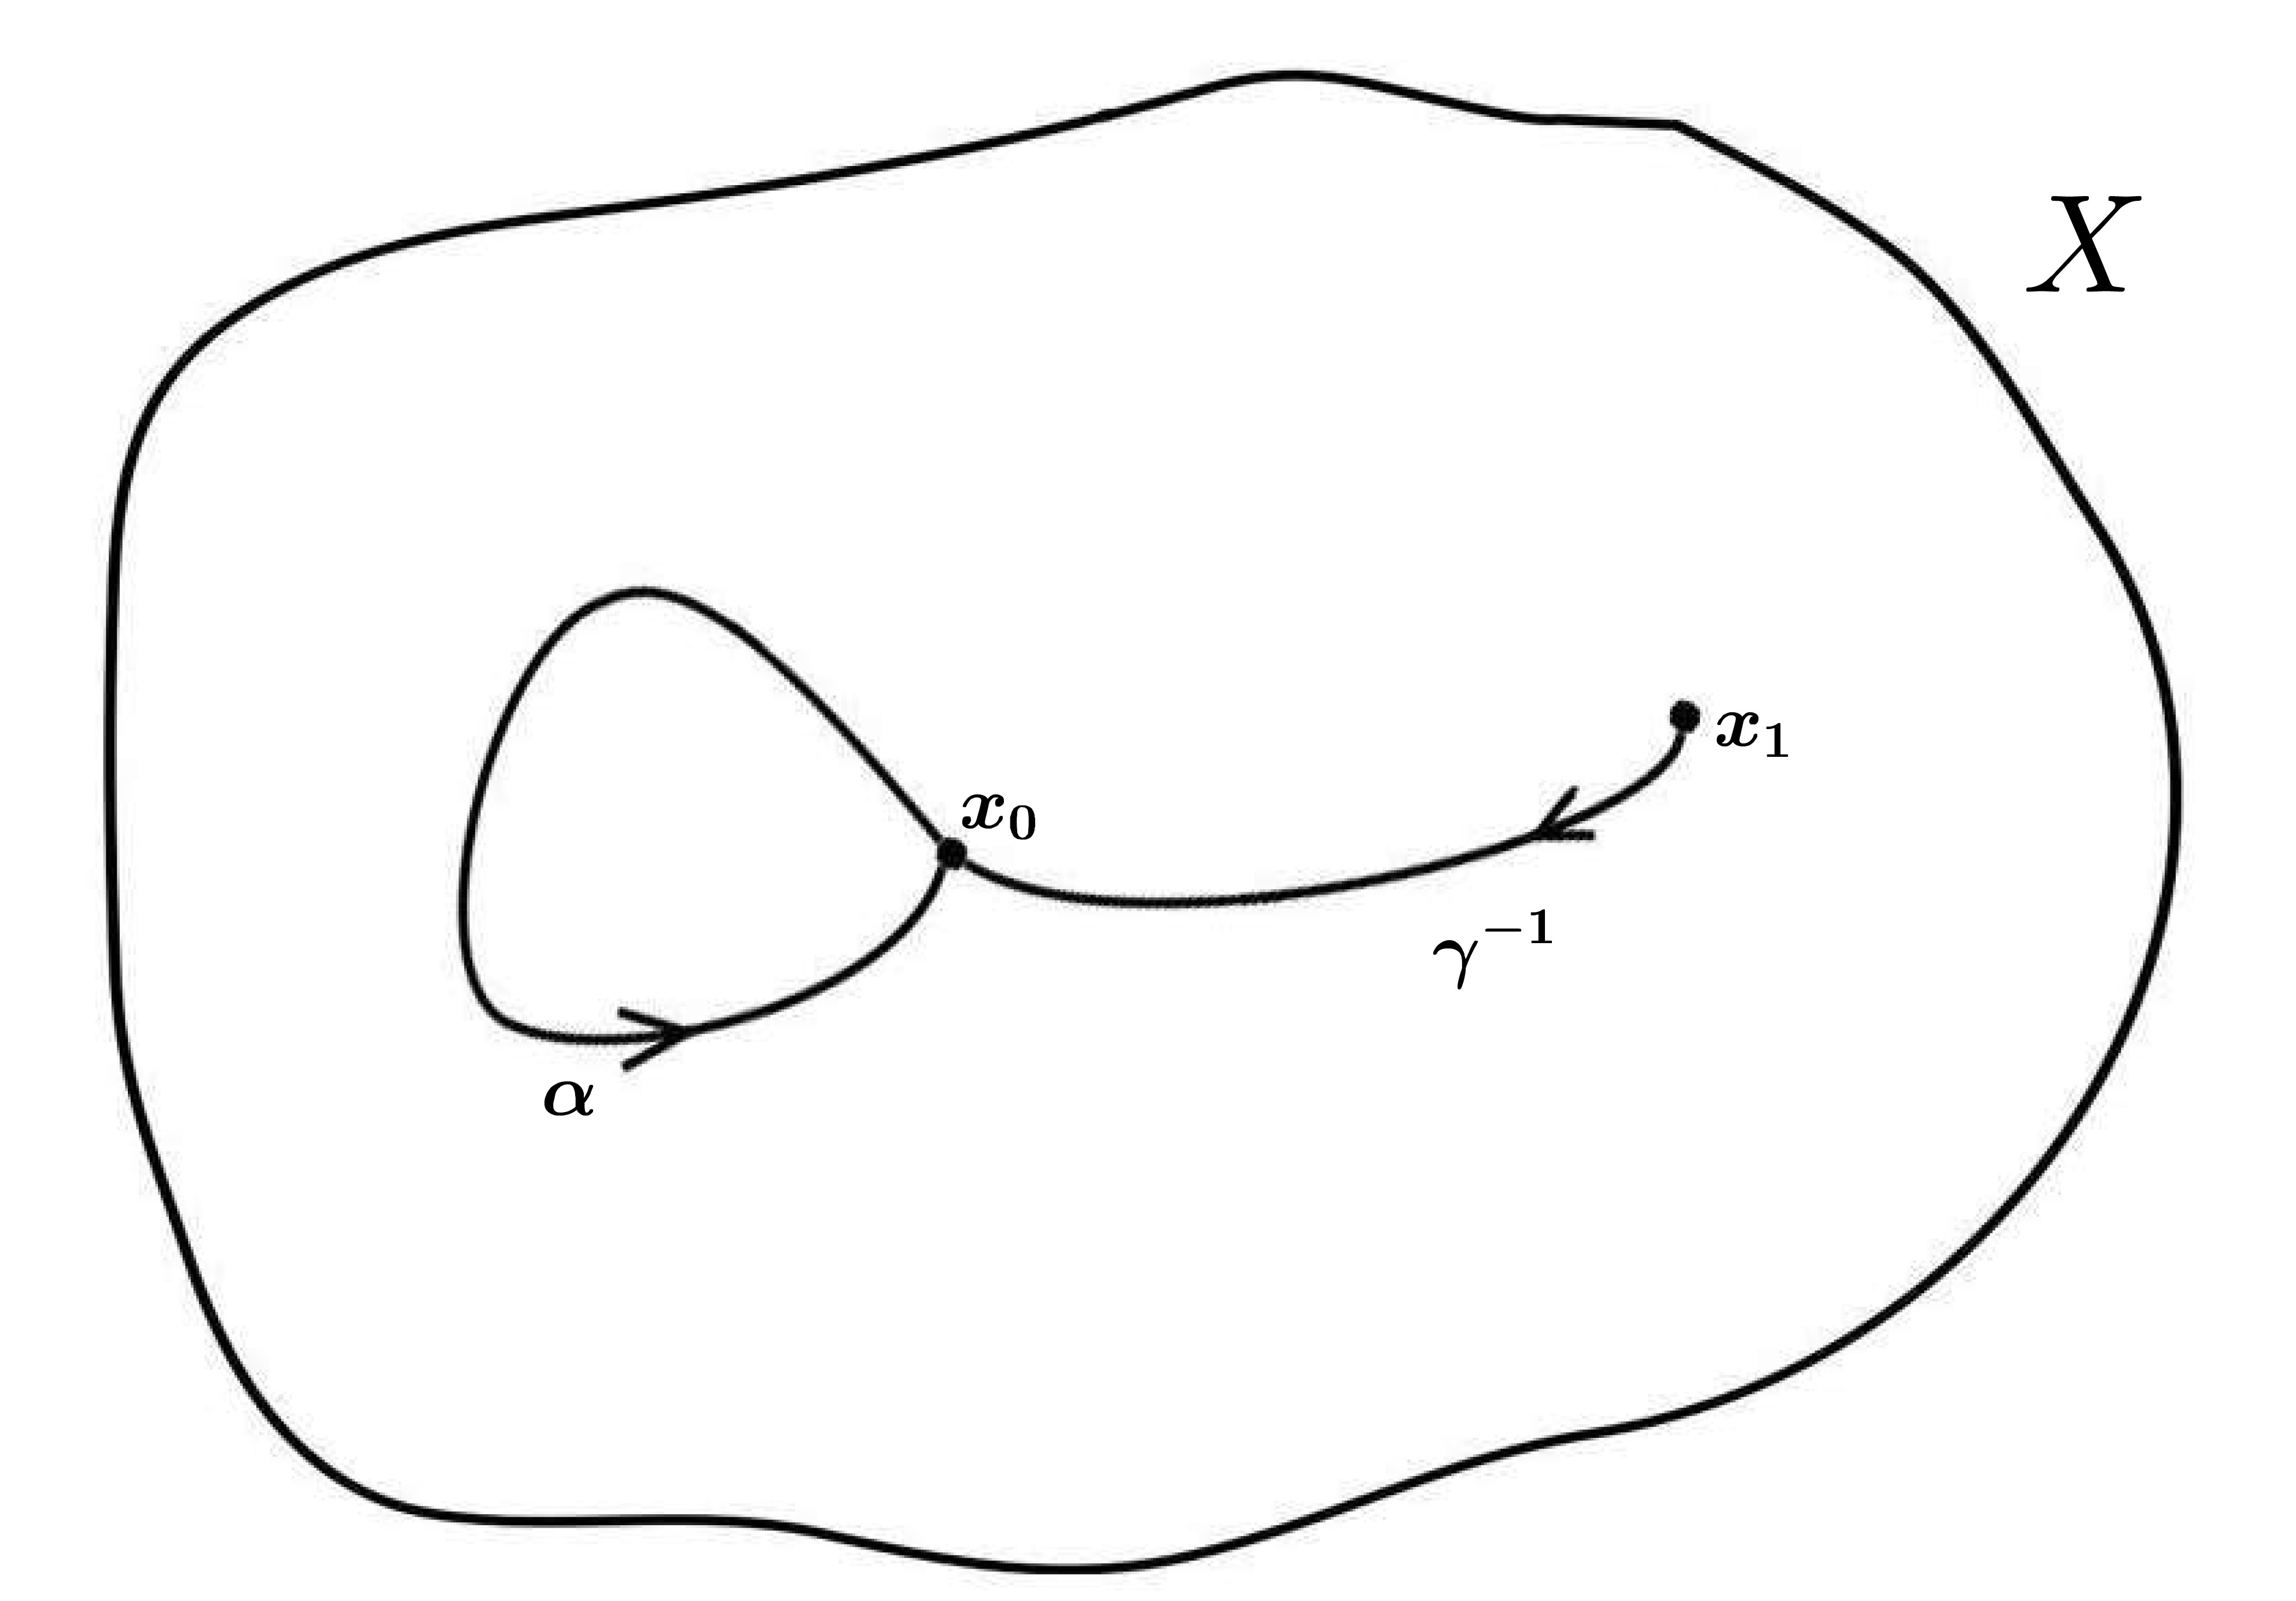
\includegraphics[width=.45\textwidth]{./images/loop.jpg}
\caption{The importance of base point}
\end{figure}



We therefore define $$ u_\gamma:\pi_1(X,x_0)\rightarrow \pi_1(X,x_1)  $$
by $u_\gamma[\alpha]=[\gamma^{-1}\ast\alpha\ast\gamma]$ that is, follow $\gamma^{-1}$ from $x_1$ to $x_0$, then follow $\alpha$ around back to $x_o$, then follow $\gamma$ back to $x_1$, all giving a loop based at $x_1$.
\begin{align*}
u_\gamma([\alpha]\ast[\beta])&=u_\gamma([\alpha\ast\beta])\\
                             &=[\gamma^{-1}\ast\alpha\ast\beta\ast\gamma]\\
                             &=[\gamma^{-1}\ast\alpha\ast\gamma\ast\gamma^{-1}\ast\beta\ast\gamma]\\
                             &=[\gamma^{-1}\ast\alpha\ast\gamma]\ast[\gamma^{-1}\ast\beta\ast\gamma]\\
                             &=u_\gamma([\alpha])\ast u_\gamma([\beta])
\end{align*}
Thus, $u_\gamma$ is a homomorphism.

Using the path $\gamma^{-1}$ from $x_1$ to $x_0$ we can define

$$u_{\gamma^{-1}}: \pi_1(X,x_1)\rightarrow \pi_1(X,x_0)$$

by $u_{\gamma^{-1}}([\alpha])=[\gamma\ast\alpha\ast\gamma^{-1}]$.\\
Now, check \begin{align*}
u_{\gamma^{-1}}u_\gamma[\alpha]=u_{\gamma^{-1}}[\gamma^{-1}\ast\alpha\ast\gamma]=[\gamma\ast\gamma^{-1}\ast\alpha\ast\gamma\ast\gamma^{-1}]=[\alpha]\\
u_{\gamma}u_{\gamma^{-1}}[\alpha]=u_{\gamma}[\gamma\ast\alpha\ast\gamma^{-1}]=[\gamma^{-1}\ast\gamma\ast\alpha\ast\gamma^{-1}\ast\gamma]=[\alpha]
\end{align*}
So, $u_\gamma$ is bijective and hence an isomorphism.
\end{proof}

\begin{definition}
A space $X$ is said to be path connected if any two points of $X$ can be joined by a path in $X$.
\end{definition}

\begin{cor}
If $X$ is a path connected space, then $\pi_1(X,x_0)$ and $\pi_1(X,x_1)$ are isomorphic groups for any pair of points $x_0,x_1\in X$.
\end{cor}

Let's look at some examples and wind up our discussion

\begin{example}
(\textbf{A simple connected space})

Suppose that a topological space $X$ is simply connected. In this case all loops with a base point $x_0$ are homotopic, resulting in one equivalence class. The result is $\pi_1(X)=0$, which is a group that consists of only the identity element.
\end{example}

\begin{example}
(\textbf{Circle})

Suppose $X=\mathbb{S}^1$. In this case there is an equivalence class for each $i\in \mathbb{Z}$, the set of integers. If $i\ge0$, then it means that the path travels $i$ times around $\mathbb{S}^1$ in the counterclockwise direction and then returns to $x_0$. If $i\le0$, then the path travels around $i$ times in in the clockwise direction. If $i=0$, then the path is equivalent to the one that remain at $x_0$ (constant loop). The fundamental group is $\mathbb{Z}$ with respect to the operation addition. If $\alpha_1$ travels $i_1$ times counterclockwise and $\alpha_2$ travels $i_2$ times counterclockwise, then $\alpha =\alpha_1\circ\alpha_2$ belongs to the class of loops that travel around $i_1+i_2$ times counterclockwise.

Consider additive inverses. If a path travels seven times around $\mathbb{S}^1$, and it is combined with a path that travels seven times in the opposite direction, the result is homotopic to the constant path (a path that remains at $x_0$). Thus, $\pi_1(\mathbb{S}^1)=\mathbb{Z}$.
\end{example}
Determining whether two given topological spaces are homeomorphic is a fundamental question in topology.

Showing two space are homeomorphic is a matter of constructing a continuous map from one to the other which has also a continuous inverse.

If we can find some topological property that holds for one topological space but not for the other, then this two spaces are not homeomorphic.

\begin{example}
(1) $[0,1]$ is not homeomorphic to $(0,1)$ since the first is compact and the second is not.
(2) $\mathbb{R}$ is not homeomorphic to $\mathbb{R}^2$ since deleting a point from $\mathbb{R}^2$ leaves a connected space and deleting a point from $\mathbb{R}$ does not.
(3) [i.] $\mathbb{R}^2$ is not homeomorphic to $\mathbb{R}^3$. Because deleting a point from $\mathbb{R}^3$ leaves a simply connected space, but deleting a point from $\mathbb{R}^2$ does not. [ii.] $S^2\ncong T$ using similar argument.
        
\end{example}
As we have seen earlier, the idea of \textbf{simple connectedness} is generalised through the \textbf{fundamental group}, which includes simple connectedness as a special case.
The condition of simple connectedness is just the condition that the fundamental group of $X$ is the trivial group.
So, the most important way of determining two spaces are not homeomorphic is by using their fundamental group. % Background Theory
%% ----------------------------------------------------------------
% Now begin the Appendices, including them as separate files

\addtocontents{toc}{\vspace{2em}} % Add a gap in the Contents, for aesthetics

\appendix % Cue to tell LaTeX that the following 'chapters' are Appendices
\clearpage  %Start a new page
\lhead{\emph{History}}  % Set the left side page header to "Symbols"
\chapter{History}


\section{Henri Poincare}
(Source: Wikipedia)

Poincar\'{e} was born on 29 April 1854 in City Ducale neighborhood, Nancy into an influential family.
\begin{figure}[hbt!]
\centering
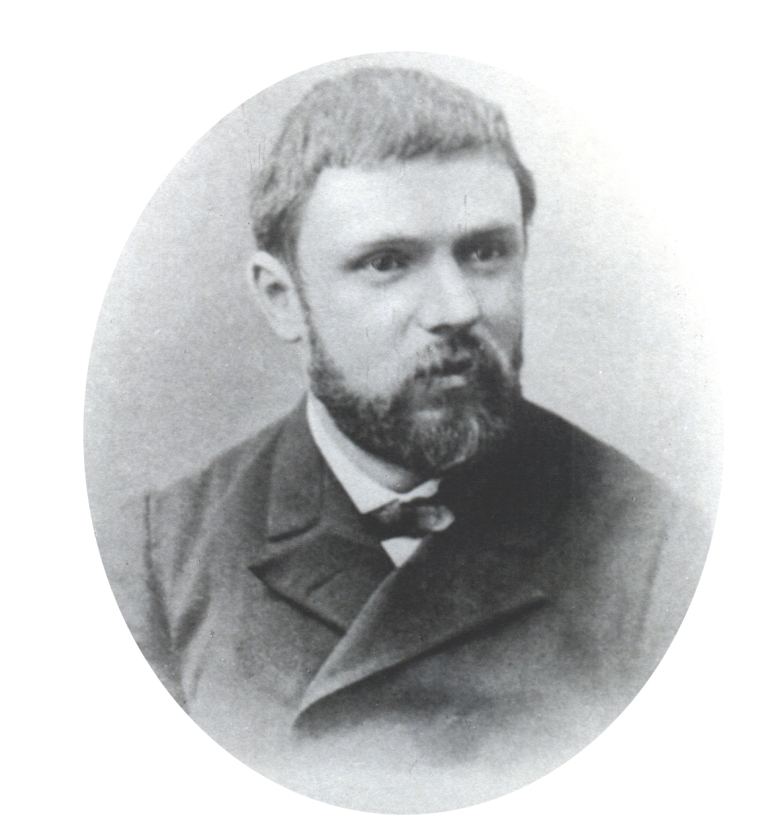
\includegraphics[width=.5\textwidth]{./images/poincare1.jpg}
\caption{Henri Poincare}\label{fig1}
\end{figure}


His father Leon Poincar\'{e} (1828-1892) was a professor of medicine at the University of Nancy. His younger sister Aline married the spiritual philosopher Emile Boutroux. Another notable member of Jules' family was his cousin, Raymond Poincar\'{e}, who would become the President of France, 1913 to 1920, and a fellow member of the Acad\'{e}mie francaise. He was raised in the Roman Catholic faith. However, he rejected Christianity in later life and became an atheist.

Henri was a precocious student who rose immediately to the top of his class, excelling in both science and letters. At age 13, his teacher told his mother that “Henri will become a mathematician... I would say a great mathematician” (Bellivier 1956: 78). During the Franco-Prussian war in 1870 the Germans occupied Nancy and the Poincar\'{e} family was obliged to billet the secretary of the civil commissar of Nancy, with whom Henri would have a round of conversation each night after dinner in order to improve his German.

In 1871, Poincar\'{e} passed the exams in letters with the grade "good" and that in science with the grade "fair". He received a zero in mathematics for answering a different question from the one that was asked, apparently having misunderstood the question. He then took the preparatory classes in mathematics and was first in his class, also first in the academic competition and first in the national competition (concours g\'{e}n\'{e}ral) in elementary mathematics. In Paris, he entered the École Polytechnique in 1873 and after graduating in 1875 (second in his class having apparently lost points for his inability to draw), entered the \'{E}cole des Mines. After brief service as a mine inspector, he submitted a dissertation on partial differential equations and he was then put in charge of the course on differential and integral calculus at the University of Caen.

In 1880, he submitted a memoir resolving a problem in the theory of differential equations to the competition for the grand prize in mathematics of the Academy of Sciences in Paris. Here for the first time he made use of non-Euclidean geometry, which was seen by most of his contemporaries as purely speculative. Poincar\'{e} married Louise Poulain d'Andecy on April 20, 1881 and was soon thereafter put on the faculty of sciences at the University of Paris. In 1886 he succeeded G. Lippmann in the chair of mathematical physics and probability. In 1896 he took the chair of mathematical astronomy and celestial mechanics, in 1902 he was named professor of theoretical electricity at the school of the post and telegraph and in 1904 professor of general astronomy at the \'{E}cole Polytechnique. Poincar\'{e} also worked at the French Bureau des Longitudes from 1893 (Galison 2003).

In 1889, Poincar\'{e} won the prize from the King of Sweden for a question posed by Weierstrass on the stability of the solar system, that is to say, the three-body (or n-body) problem in classical mechanics. Despite a mathematical error which he discovered at the last moment (after questions raised by the Swedish mathematician Lars Edvard Phragm\'{e}n) and frantically corrected, the work was important for its use of topology and as a founding document in chaos theory, for Poincar\'{e} showed that in general, the stability of such systems cannot be demonstrated. It is also in this context that he proved his famous recurrence theorem.

Poincar\'{e} joined the French Academy of Sciences in 1887 and became its president in 1906. On the basis of his three books on philosophical and general problems in science, he was elected to the Académie Française in 1908. He also became a corresponding member of many international scientific organizations. Poincar\'{e}'s extensive correspondence demonstrates the extent of his relations with the scientific community of his time (Nabonnand 1999; Walter 2007). His travel included a trip to America to give a lecture at the St. Louis World's Fair in 1904. He also co-signed a report that played an important role in the rehabilitation of Dreyfus.


\begin{figure}[hbt!]
\centering
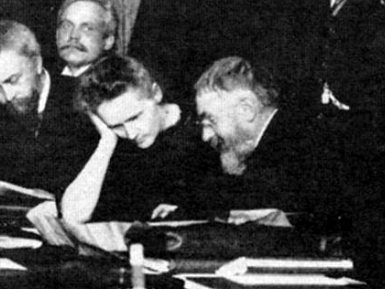
\includegraphics[width=.5\textwidth]{./images/solvay.jpg}
\caption{Henri Poincare with Marie Curie on the 1911 Solvay conference}\label{fig1}
\end{figure}

Poincar\'{e} is also famous for his 1904 conjecture concerning the topology of three-dimensional spheres, which remained one of the major unsolved problems in mathematicsuntil very recently, the Russian mathematician Grigori Perelman succeeded in demonstrating it nearly one hundred years later. Poincaré lectured on contemporary mathematical physics for years and was very much abreast of current developments. In all he published over five hundred scientific papers and over thirty books. He died from an embolism, at age fifty eight, on 17 July 1912, and was buried inside the Poincare family vault in the cemetery of Montparnasse, Paris.
\clearpage

	% Appendix Title
\addtocontents{toc}{\vspace{2em}}  % Add a gap in the Contents, for aesthetics
\backmatter
\newpage
%% ----------------------------------------------------------------
\label{Bibliography}
\begin{thebibliography}{6}
{\small

\item[\textbf{[1]}]
Hatcher, A. \textit{Algebraic Topology.} Cambridge, England: Cambridge University Press, 2006.

\item[\textbf{[2]}]
Sidney A. Morris
\textit{Topology without Tears.}. 2nd ed.

\item[\textbf{[3]}]
James Munkres \textit{Topology,} Second Edition.

\item[\textbf{[4]}]
Marlow Anderson, Todd Fiel \textit{A  First Course in Abstract Algebra} 2nd ed.

\item[\textbf{[5]}]
Joseph Gallian \textit{Contemporary abstract algebra} 8th ed.

\item[\textbf{[6]}]
Fraleigh, J. B.
\textit{A First Course in Abstract Algebra}. 7th ed.
Pearson, NJ, 2003.


\item[\textbf{[7]}]
  I.M singer \textit{Lecture notes in elementary topology and geometry}.

\item[\textbf{[8]}]
Joseph Rotman \textit{An Introduction to Algebraic Topology}.

\item[\textbf{[9]}]
Seymour Lipschutz \textit{Genereal Topology} (1965).

\item[\textbf{[10]}]
 Marvin  and Harper \textit{Algebraic Topology A First Course} (1981).


}
\end{thebibliography}
	% Appendix Title

\end{document}  % The End
%% ----------------------------------------------------------------
